\documentclass[10pt,twoside]{report}

%images
    \usepackage{graphicx} %?
    \usepackage{transparent} %images opacity
    \usepackage{tikz} %draw figures
        \newcommand{\bolverm}[0]{\tikz\draw[deep_carmine,fill=white] (0,0) circle (.5ex);}
        \newcommand{\bolverde}[0]{\tikz\draw[tropical_rain_forest,fill=white] (0,0) circle (.5ex);}
        \newcommand{\bolazul}[0]{\tikz\draw[absolute_zero,fill=white] (0,0) circle (.5ex);}
        \newcommand{\formell}[0]{\textbf{[F]}}
        \newcommand{\informell}[0]{\textbf{[I]}}
    \usepackage[pages=some]{background} %set page background as image, colour, ect
    \usepackage{etoolbox} %icons for chapter, section and subsection titles
        \newrobustcmd{\icongit}{\includegraphics[height=10pt]{figures/icon/icon_git.eps}}
        \newrobustcmd{\iconcpp}{\includegraphics[height=10pt]{figures/icon/icon_cpp.eps}}
        \newrobustcmd{\iconmysql}{\includegraphics[height=10pt]{figures/icon/icon_mysql.eps}}
        \newrobustcmd{\iconvs}{\includegraphics[height=10pt]{figures/icon/icon_vs.eps}}

%maths language
    %\usepackage[fleqn]{amsmath,empheq}
    \usepackage[fleqn]{mathtools}
        \DeclareMathOperator{\rot}{rot} %define new maths symbol
        \DeclareMathSizes{10pt}{10pt}{5pt}{5pt} %declare maths size
    \usepackage{cancel} %cancel equations terms
    \usepackage{chemfig} %chemistry equations
    \usepackage[version=4]{mhchem} %?
    \usepackage{esvect} %arrows above maths letters

%tables
    \usepackage{booktabs} %?
    \usepackage{array} %?
    \usepackage{longtable,tabu} %for long tables which splits into different pages
        \newcolumntype{C}[1]{>{\centering\arraybackslash}p{#1}} %centering columns
    \usepackage{tabularx} %set different columns width in the same table
    \usepackage{multicol} %merge several columns
    \usepackage{blindtext} 
    \usepackage{multirow} %merge several rows
    \usepackage{hhline} %double horizontal lines

%universal info
    \usepackage[utf8]{inputenc} %encoding type
    \usepackage[portuguese, english]{babel} %document language
    \usepackage{xcolor} %colour package
    \usepackage{color} %colour package 
        %colors
        \definecolor{tropical_rain_forest}{HTML}{08605F}
        \definecolor{deep_carmine}{HTML}{A4243B}
        \definecolor{absolute_zero}{HTML}{0051BA}
        \definecolor{saffron}{HTML}{EFB22D}
        \definecolor{sunset_orange}{HTML}{f25f5c}
        \definecolor{light_gray}{HTML}{D1D2D4}
        \definecolor{anti_flash_white}{HTML}{F2F2F3}
        \definecolor{toolbox}{HTML}{717ec3}
        \definecolor{indian_red}{HTML}{c95d63} 
        \definecolor{xanadu}{HTML}{708b75}
        \definecolor{french_plum}{HTML}{861657}
        \definecolor{ref_2}{HTML}{DFB9BF}
        \definecolor{ref_1}{HTML}{97C3A4}
        \definecolor{honey_gold}{HTML}{e79001}
        \definecolor{davys_grey}{HTML}{545454}

        \definecolor{textcolor}{HTML}{545454}
    \usepackage{datetime} %get current day, month and year
    \usepackage{dashrule} %draw dashed lines
    \usepackage{ar} %aspect ratio symbol
    \usepackage{eurosym} %euro symbol (€)
    \usepackage{sectsty} %edit section title appearance
    \usepackage{titlesec} %change titles appearance with a single command
    \PassOptionsToPackage{obeyspaces}{url} %respect \href spaces
    \usepackage[font={color=textcolor}]{caption} %change figures captions
    \usepackage{hyperref} %hide boxes around hyperlink
        \hypersetup{colorlinks, %color text of links and anchors, eliminates borders around links
        linkcolor=textcolor,        %color for normal internal links
        anchorcolor=textcolor,      %color for anchor text
        citecolor=textcolor,        %color for bibliographical citations
        filecolor=textcolor,        %color for URLs which open local files
        menucolor=textcolor,        %color for Acrobat menu items
        pagecolor=textcolor,        %color for links to other pages
        urlcolor=textcolor,         %color for linked URLs
        bookmarks=true,         %create PDF bookmarks
        bookmarksopen=false,    %don't expand bookmarks
        bookmarksnumbered=true, %number bookmarks
        pdftitle={mybible},
        pdfauthor={duarte vicente drumond},
        pdfsubject={guia de um terráqueo para viver bem na lua},
        pdfkeywords={self},
        pdfstartview=FitV,
        pdfdisplaydoctitle=true}
        \makeatletter
        \newcommand\HREF[2]{\hyper@linkurl{#2}{#1}}
        \makeatother
    \usepackage{float} %positioning figures, tables, etc
    \usepackage{mVersion} %read .sty files
        \usepackage{my_preamble}
    \usepackage{scrextend} %add margin to a text box
    \usepackage{cleveref} %cross referencing
        \newcommand{\genref}[1]{(\cref{#1})}
    \usepackage{tcolorbox} %colour package
    \usepackage[final]{pdfpages} %include pdfs

%text setting
    \usepackage[verbose, right=25mm, bottom=25mm, left=25mm, top=20mm,marginparwidth=3cm]{geometry} %set margins
    \usepackage[defaultsans]{opensans} %font-family and size
        \renewcommand{\sfdefault}{fos} %define font Open Sans (fos) as the default sans serif font family
        \renewcommand\familydefault{\sfdefault} %define default font family as sans serif font family
        \def\chapterfont{\usefont{T1}{fos}{b}{cl}\fontsize{25pt}{25pt}\selectfont}
        \def\sectionfont{\usefont{T1}{fos}{b}{cl}\fontsize{15pt}{15pt}\selectfont}
        \def\subsectionfont{\usefont{T1}{fos}{b}{cl}\fontsize{12pt}{12pt}\selectfont}
        \def\subsubsectionfont{\usefont{T1}{fos}{b}{cl}\fontsize{10pt}{10pt}\selectfont}
        \def\Big{\usefont{T1}{fos}{b}{cl}\fontsize{16pt}{16pt}\selectfont}
        \def\normal{\usefont{T1}{fos}{m}{m}\fontsize{10pt}{10pt}\selectfont}
        \def\normalbold{\usefont{T1}{fos}{b}{m}\fontsize{10pt}{10pt}\selectfont}
        \def\normalitalic{\usefont{T1}{fos}{m}{it}\fontsize{10pt}{10pt}\selectfont}
        \DeclareRobustCommand\ebseries{\fontseries{eb}\selectfont}
        \DeclareRobustCommand\sbseries{\fontseries{sb}\selectfont}
        \DeclareRobustCommand\ltseries{\fontseries{l}\selectfont}
        \DeclareRobustCommand\clseries{\fontseries{cl}\selectfont}
        \DeclareTextFontCommand{\texteb}{\ebseries}
        \DeclareTextFontCommand{\textsb}{\sbseries}
        \DeclareTextFontCommand{\textlt}{\ltseries}
        \DeclareTextFontCommand{\textcl}{\clseries}
    \usepackage[document]{ragged2e} %justify, center, left and right align text
    \usepackage[normalem]{ulem} %underline text
    \usepackage[shortlabels]{enumitem} %lists
        \newlist{Enumerate}{enumerate}{9}  %new list type called Enumerate
            \setlist[Enumerate,1]{label=\arabic*.}
            \setlist[Enumerate,2]{label=\Roman*.}
            \setlist[Enumerate,3]{label=\Alph*.}
            \setlist[Enumerate,4]{label=\roman*.}
            \setlist[Enumerate,5]{label=\alph*.}
            \setlist[Enumerate,6]{label=\arabic*.}
            \setlist[Enumerate,7]{label=\Roman*.}
            \setlist[Enumerate,8]{label=\Alph*.}
            \setlist[Enumerate,9]{label=\roman*.}

        \setlist[enumerate]{label*=\arabic*.} %edit list enumerate
    \usepackage{setspace} %line spacing
        \renewcommand{\baselinestretch}{1.5} %space between normal text lines
        \setlength{\parskip}{1.5mm} %space between paragraphs
        \setlength{\parindent}{20mm} %?
    
    %titles format
        \titleformat{\chapter}[display]{\sffamily}{}{25pt}{\chapterfont} %chapter title appearance
        \titleformat{\section}{\sectionfont}{\thesection}{15pt}{} %section title appearance
        \titleformat{\subsection}{\subsectionfont}{\thesubsection}{12pt}{} %subsection title appearance
        \titleformat{\subsubsection}{\subsubsectionfont}{\thesubsubsection}{10pt}{} %subsection title appearance
    \usepackage{soul} %highlight text
        \DeclareRobustCommand{\hlgrey}[1]{{\sethlcolor{anti_flash_white}\hl{#1}}} %change highlight color when using \hlgrey to grey

    %others
        \usepackage{accents}
            \newcommand{\phonetics}[3]{ $\underset{\textit{[#2]} \, \textit{#3}}{\text{#1}}$ }
  
%header and footer setting
    \usepackage{fancyhdr} %page headers and footers
    \fancypagestyle{plain}{
        \fancyhf{} %clear all header and footer fields
        \fancyfoot[C]{\color{textcolor}\sffamily\fontsize{9pt}{9pt}\selectfont\thepage} %define the center footer
        \renewcommand{\headrulewidth}{0pt}
        \renewcommand{\footrulewidth}{0pt}
    }

%table of contents (ToC) setting
    \addto\captionsportuguese{\renewcommand{\contentsname}{Índice}} %change title name in portuguese language to "índice"
    \usepackage{tocloft} %edit table of contents design
    \renewcommand{\cftdotsep}{7} %input a number for dot separation or \cftnodots to remove dots
    \renewcommand{\cfttoctitlefont}{\Big} %change title font size, type and family
    \renewcommand{\cftchapfont}{\normalbold} %change section font size, type and family
    \renewcommand{\cftchappagefont}{\normalbold} %change section page number font size, type and family
    \renewcommand{\cftchapaftersnumb}{ } %change space between section number and name
    %\renewcommand{\cftsecfont}{\normal} %change section font size, type and family
    %\renewcommand{\cftsecpagefont}{\normal} %change section page number font size, type and family
    \renewcommand{\cftsecaftersnumb}{ } %change space between section number and name
    %\renewcommand{\cftsubsecfont}{\normal} %change subsection font size, type and family
    %\renewcommand{\cftsubsecpagefont}{\normal} %change subsection page number font size, type and family
    \renewcommand{\cftsubsecaftersnumb}{ } %change space between subsection number and name
    %\renewcommand{\cftsubsubsecfont}{\normal} %change subsubsection font size, type and family
    %\renewcommand{\cftsubsubsecpagefont}{\normal} %change subsubsection page number font size, type and family
    \renewcommand{\cftsubsubsecaftersnumb}{ } %change space between subsubsection number and name
    
    %\setcounter{secnumdepth}{0} %hide sections and subsections numbering

%glossary
    \usepackage[nopostdot,acronym]{glossaries} %make glossary
        \makeglossaries
        \glsenablehyper
        \renewcommand{\glsnamefont}{\sffamily}

%nomenclature
    % \usepackage{nomencl} %make glossary
    %     \makenomenclature
    %     \renewcommand{\nomname}{Lista de Símbolos}
    % \usepackage{etoolbox}
    %     \renewcommand\nomgroup[1]{
    %         \item[\bfseries
    %             \ifstrequal{#1}{T}{Tecnologias}
    %         ]
    %     }

%external files input
    \usepackage{fancyvrb} %print .txt files
    \usepackage{listings} %print files
        \lstdefinelanguage{JavaScript}{
            keywords={break, case, catch, continue, debugger, default, delete, do, else, false, finally, for, function, if, in, instanceof, new, null, return, switch, this, throw, true, try, typeof, var, void, while, with},
            morecomment=[l]{//},
            morecomment=[s]{/*}{*/},
            morestring=[b]',
            morestring=[b]",
            ndkeywords={class, export, boolean, throw, implements, import, this},
            sensitive=true
        }
        %define appearance for all the files
            \lstdefinestyle{basic}{frame=ltb,
                %space and placement
                    aboveskip = 3mm, %distance between the box and the previous line
                    belowskip = 0mm, %distance between the box and the next line
                %appearance
                    basicstyle = \ttfamily\small, %edit font appearance
                    commentstyle = \color{tropical_rain_forest}, %edit comments appearance
                    stringstyle = \color{deep_carmine}, %edit appearance of words inside ''
                    %edit keywords style
                        %default keyword style
                            classoffset = 0, 
                            morekeywords={checkout},keywordstyle=\color{absolute_zero},
                        %keyword style 1
                            classoffset = 1, 
                            morekeywords={data},keywordstyle=\color{sunset_orange},
                        classoffset = 0,
                sensitive=true,
                framerule=0pt, %edit frame thickness around box 
                backgroundcolor = \color{anti_flash_white}, %background colour
                showstringspaces=false,
                columns=flexible,
                framextopmargin=0cm,
                framexleftmargin=1cm,
                xleftmargin=1.2cm,
                xrightmargin=1.2cm,
                framexbottommargin=0cm,
                numbers=right,
                numberstyle=\tiny\color{black},
                breaklines=true,
                breakatwhitespace=true,
                tabsize=1
            }
%bibliography
    \usepackage{biblatex}
        \addbibresource{bibliography.bib}
        \renewbibmacro{in:}{}

        \DeclareFieldFormat{bibentrysetcount}{\mkbibparens{\mknumalph{#1}}}
        \DeclareFieldFormat{labelnumberwidth}{\mkbibbrackets{#1}}

        \defbibenvironment{bibliography}
        {\list
            {\printtext[labelnumberwidth]{%
            \printfield{prefixnumber}%
            \printfield{labelnumber}}}
            {\setlength{\labelwidth}{\labelnumberwidth}%
            \setlength{\leftmargin}{\labelwidth}%
            \setlength{\labelsep}{\biblabelsep}%
            \addtolength{\leftmargin}{\labelsep}%
            \setlength{\itemsep}{\bibitemsep}%
            \setlength{\parsep}{\bibparsep}}%
            \renewcommand*{\makelabel}[1]{\hss##1}}
        {\endlist}
        {\item}

%extra commands
    \newcommand{\code}[1]{\ttfamily\hlgrey{#1}\sffamily }
    \newcommand{\cpp}[0]{\iconcpp \, C++}
    \newcommand{\mysql}[0]{ \iconmysql \, MySQL }
    \newcommand{\vs}[0]{ \iconvs \, Visual Studio }
    \newcommand{\translation}[1]{\footnotesize \quad\textit{#1}\normalsize}

\begin{document}

    \color{textcolor} %text color
    \pagestyle{plain} %no header, footer with centred number
    \pagenumbering{roman} %define page numbering type: roman, arabic and gobble (disable page numbering)
    \justify %justify all document; commands: \RaggedRight, \RaggedLeft, \Centering, \justify 

    %Cover
        \thispagestyle {empty} %removes page numbering

\begin{flushleft}
    
    \vspace*{\fill}
    
    {\Big Deutschkurs}\par
    
    {por duarte vicente drumond}\par\vspace{1cm}
    
    {24.10.2021  - \the\day.\the\month.\the\year}\par\vspace{1cm}
    
    \vspace*{\fill}
        
\end{flushleft}
        
        \cleardoublepage %blank page printed if odd number page
        
    %Dedication
        %\input{dedication.tex}
        %\cleardoublepage %blank page printed if odd number page

    %Abstract
        %Put abstract in table of contents (ToC)
        %\phantomsection
        %\addcontentsline{toc}{section}{Resumo}
        %\input{abstract.tex}
        %\cleardoublepage %blank page printed if odd number page

    %Table of Contents (ToC)
        \tableofcontents
        \cleardoublepage %blank page printed if odd number page

    %Glossary
        \newglossaryentry{version control}{
    name=version control,
    description={Version control systems are a category of software tools that help a software team manage changes to source code over time. Version control software keeps track of every modification to the code in a special kind of database. If a mistake is made, developers can turn back the clock and compare earlier versions of the code to help fix the mistake while minimizing disruption to all team members.}
}

\newglossaryentry{git}{
    name=Git\texttrademark,
    description={\Gls{version control} system for tracking changes in computer files and coordinating work on those files among multiple people. It is primarily used for source-code management in software development, but it can be used to keep track of changes in any set of files.}
}

\newglossaryentry{ddr}{
    name=DDR,
    description={Dose diária recomendada}
}

\newacronym{peg}{PEG}{polyethylene glycol}
\newacronym{sls}{SLS}{sodium lauryl sulfate}
\newacronym{sles}{SLES}{sodium laureth sulfate}

        %Put Glossary's section in Table of contents (ToC)
            \phantomsection
            \addcontentsline{toc}{section}{\glossaryname}
            \printglossary[type=\acronymtype]
            \printglossary
            \cleardoublepage

    %Starts a new type of numbering
        \setcounter{page}{1}
        \pagenumbering{arabic}

    %Chapters
        \chapter{Start auf Deutsch}\label{chapter:start_auf_deutsch}

    \section{das Alphabet / o alfabeto}\label{section:deutsch:alphabet}    

        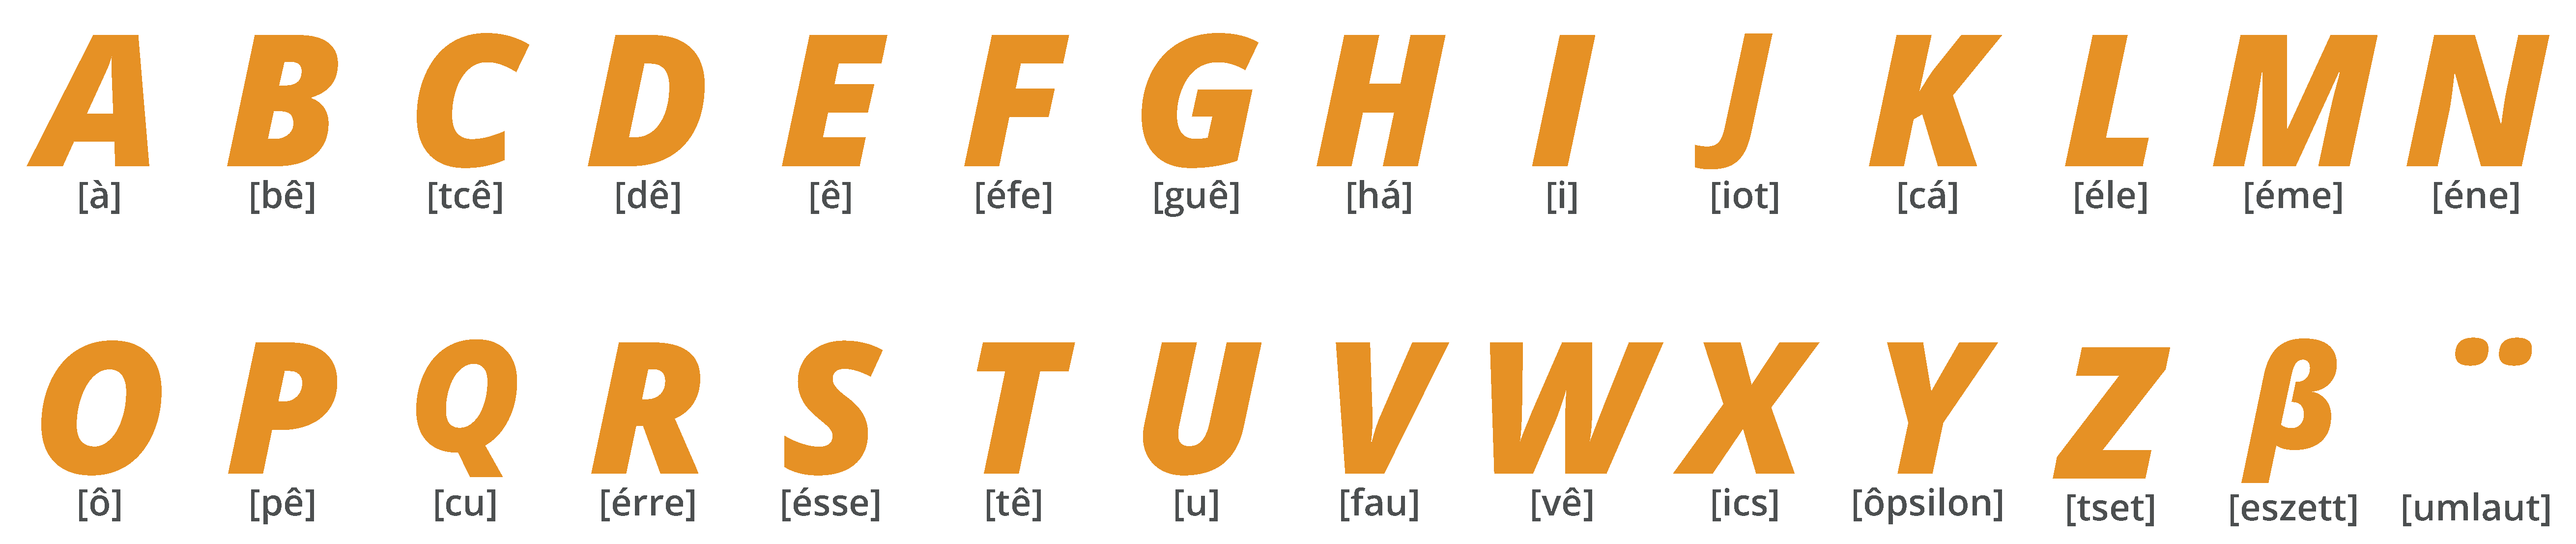
\includegraphics[width=.9\linewidth]{figures/dasAlphabet.eps}

        Können Sie das buchstabieren bitte? \translation{Pode soletrar isso, por favor?}

    \section{Begrüßen und verabschieden / Saudações e despedidas}\label{section:begrussenverabschieden}

        \begin{multicols}{2}
            \begin{itemize}[topsep=0pt,itemsep=4pt,parsep=0pt]
                \item[-] Hallo \translation{olá}
                \item[-] Guten Morgen \translation{bom dia}
                \item[-] Guten Tag \translation{boa tarde}
                \item[-] Guten Abend \translation{boa noite}
                \item[-] Gute Nacht \translation{boa noite (despedir-se antes de ir dormir)}
                \item[-] Grüß Gott \translation{saudação religiosa}
                \item[-] Servus \translation{olá} 
            \end{itemize}
        \vfill\null
        \columnbreak
            \begin{itemize}[topsep=0pt,itemsep=4pt,parsep=0pt]
                \item[-] Auf Wiedersehen \translation{até nos vermos novamente (pessoalmente)}
                \item[-] Auf Wiederschauen \translation{até te contemplar novamente}
                \item[-] Auf Wiederhören \translation{até nos ouvirmos novamente (chamada telefónica)}
                \item[-] Tschüs \translation{tchau}
                \item[-] bis bald \translation{até breve}
                \item[-] bis spätter \translation{até mais tarde}
                \item[-] Servus \translation{adeus}
                \item[-] Baba \translation{adeus (em Österreich)}  
            \end{itemize}
        \end{multicols}

    \section{das Datum / a data}\label{section:deutsch:dasdatum}

        Donnerstag, den 7. März 2019\\
        Heute haben wir Donnerstag, den siebten März zweintausendundneunzehn\\

    \section{vorstellen / apresentar}\label{section:deutsch:vorstellen}

        \subsection{ich vorstellen / apresentar-me}\label{subsection:deutsch:ich_vorstellen}
            
            \begin{itemize}[topsep=0pt,itemsep=4pt,parsep=0pt]
                \item[-] Wie heißt du? \translation{Como te chamas?}
                    \begin{itemize}
                        \item[-] Ich heiße Duarte. \translation{Eu chamo-me Duarte.}
                    \end{itemize}
                \item[-] Wer bist du? \translation{Quem és?}
                    \begin{itemize}
                        \item[-] Ich bin Duarte. \translation{Eu sou o Duarte.}
                    \end{itemize}
                \item[-] Woher kommst du? \translation{Donde és?}
                    \begin{itemize}
                        \item[-] Ich komme aus Funchal, aus Portugal. \translation{Eu sou do Funchal, Portugal.}
                    \end{itemize}
                \item[-] Wo wohnst du? \translation{Onde moras?}
                    \begin{itemize}
                        \item[-] Ich wohne in Lissabon. \translation{Eu moro em Lisboa.}
                    \end{itemize}
                \item[-] Welche Sprachen sprechst du? \translation{Que línguas falas?}
                    \begin{itemize}
                        \item[-] Ich spreche Portugiesisch. \translation{Eu falo português.}
                    \end{itemize}
            \end{itemize}

        \subsubsection{die Länder / os países}\label{subsubsection:deutsch:ich_vorstellen:lander}

            \begin{longtabu}to \textwidth {>{\scriptsize}X[0.3,m] >{\scriptsize}X[1,m] >{\scriptsize}X[1,m] >{\scriptsize}X[1,m] >{\scriptsize}X[1,m] >{\scriptsize}X[1,m] >{\scriptsize}X[1,m]}
                \toprule
                & \multirow{2}{*}{\textbf{\normalsize Land}} & \multirow{2}{*}{\textbf{\normalsize Sprache}} & \multicolumn{3}{c}{\textbf{Nationalität}} & \multirow{2}{*}{\textbf{\normalsize Adjektiv}} \\ 
                & & & \textsb{Maskulinum (der)} & \textsb{Femininum (die)} & \textsb{Plural (die)} &\\ 
                \toprule \endhead
                    
\includegraphics[width=0.5\linewidth]{figures/lander/egypt.png} & Ägypten & Arabisch & Ägypter & Ägypterin & Ägypter & ägyptisch\\ \hline
                    
\includegraphics[width=0.5\linewidth]{figures/lander/algeria.png} & Algerien & Arabisch & Algerier & Algerierin & Algerier & algerisch \\ \hline
                    
\includegraphics[width=0.5\linewidth]{figures/lander/china.png} & China & Chinesisch & Chinese & Chinesin & Chinesen & chinesisch \\ \hline
                    
\includegraphics[width=0.5\linewidth]{figures/lander/germany.png} & Deutschland & Deutsch & Deutsche & Deutsche & Deutschen & deutsch \\ \hline
                    
\includegraphics[width=0.5\linewidth]{figures/lander/france.png} & Frankreich & Französisch & Franzose & Französin & Franzosen & französisch \\ \hline
                    
\includegraphics[width=0.5\linewidth]{figures/lander/united-kingdom.png} & Großbritannien & Englisch & Brite & Britin & Briten & britisch \\ \hline
                    
\includegraphics[width=0.5\linewidth]{figures/lander/italy.png} & Italien & Italienisch & Italiener & Italienerin & Italiener & italienisch \\ \hline
                    
\includegraphics[width=0.5\linewidth]{figures/lander/japan.png} & Japan & Japanisch & Japaner & Japanerin & Japaner & japanisch \\ \hline
                    
\includegraphics[width=0.5\linewidth]{figures/lander/lebanon.png} & der Libanon & Arabisch & Libanese & Libanesin & Libanesen & libanesisch \\ \hline
                    
\includegraphics[width=0.5\linewidth]{figures/lander/austria.png} & Österreich & Deutsch & Österreicher & Österreicherin & Österreicher & österreichisch \\ \hline
                    
\includegraphics[width=0.5\linewidth]{figures/lander/poland.png} & Polen & Polnisch & Pole & Polin & Polen & polnisch \\ \hline
                    
\includegraphics[width=0.5\linewidth]{figures/lander/portugal.png} & Portugal & Portugiesisch & Portugiese & Portugiesin & Portugiesen & portugiesisch \\ \hline
                    
\includegraphics[width=0.5\linewidth]{figures/lander/russia.png} & Russland & Russisch & Russe & Russin & Russen & russisch \\ \hline
                    
\includegraphics[width=0.5\linewidth]{figures/lander/switzerland.png} & die Schweiz & Rätoromanisch & Schweizer & Schweizerin & Schweizer & schweizerisch \\ \hline
                    
\includegraphics[width=0.5\linewidth]{figures/lander/spain.png} & Spanien & Spanisch & Spanier & Spanierin & Spanier & spanisch \\ \hline
                    
\includegraphics[width=0.5\linewidth]{figures/lander/turkey.png} & die Türkei & Türkisch & Türke & Türkin & Türken & türkisch \\ \hline
                    
\includegraphics[width=0.5\linewidth]{figures/lander/united-states.png} & die USA & Englisch & Amerikaner & Amerikanerin & Amerikaner & amerikanisch \\
                \toprule
            \end{longtabu}
            Quando o país é precedido pela preposição \phonetics{aus}{àu-ze}{de}, o artigo do país (quando o tem) muda para \phonetics{dem}{dém}{} se for masculino, para \phonetics{der}{dé-a}{} se for feminino, para \phonetics{den}{dén}{} se for plural ou não se põe nada se o país não tiver artigo.

    \pagebreak\section{im Café / no café}\label{section:deutsch:im_cafe}
    
        \begin{multicols}{3}
            \textbf{der Wortschatz}
            \begin{itemize}[topsep=0pt,itemsep=4pt,parsep=0pt]
                \item[-] viel \translation{muito}
                \item[-] wenig \translation{pouco}
                \item[-] mit \translation{com}
                \item[-] ohne \translation{sem}
                \item[-] gern \translation{gostar de}
                \item[-] lieber \translation{preferir}
                \item[-] zusammen \translation{junto}
                \item[-] getrennt \translation{separado} 
            \end{itemize}
        \vfill\null
        \columnbreak
            \textbf{die Verben}
            \begin{itemize}[topsep=0pt,itemsep=4pt,parsep=0pt]
                \item[-] trinken \translation{beber}
                \item[-] nehmen \translation{tomar}
                \item[-] möchten \translation{desejar/querer (conjuntivo do verbo mögen)}
                \item[-] zahlen \translation{pagar}
                \item[-] bestellen \translation{encomendar} 
            \end{itemize}
        \vfill\null
        \end{multicols}

        \subsection{das Gespräche / o diálogo}\label{subsection:deutsch:im_cafe:das_gesprache}

            \begin{multicols}{2}
                \textbf{etwas bestellen}
                \begin{itemize}[topsep=0pt,itemsep=4pt,parsep=0pt]
                    \item[-] \textsb{Kellner:} Guten Morgen! Was möchten Sie trinken?
                    \item[-] \textsb{A:} Ich möchte Tee mit Zucker, bitte.
                    \item[-] \textsb{Kellner:} Und Sie? Was möchten Sie trinken? Kaffe oder Tee?
                    \item[-] \textsb{B:} Ich trinke lieber Kaffe mit viel Zucker, bitte.
                    \item[-] \textsb{Kellner:} Was nehmen/trinken Sie?
                    \item[-] \textsb{C:} Ich nehme Kaffe mit wenig Milch, bitte.
                \end{itemize}
            \vfill\null
            \columnbreak
                \textbf{zahlen}
                \begin{itemize}[topsep=0pt,itemsep=4pt,parsep=0pt]
                    \item[-] \textsb{A:} Wir möchten bitte zahlen. / Wir möchten zahlen bitte. 
                    \item[-] \textsb{Kellner:} Zusammen oder getrennt?
                    \item[-] \textsb{B:} Zusammen, bitte.
                    \item[-] \textsb{Kellner:} Hmmm... Zwei Kaffee und eins Tee... Das macht 8,60\euro.
                    \item[-] \textsb{B:} Hier, bitte.
                    \item[-] \textsb{Kellner:} Danke! Auf Wiedersehen!
                \end{itemize}
            \vfill\null
            \end{multicols}

        \subsection{gern, lieber, möchten}\label{subsection:deutsch:im_cafe:gern_lieber_mochten}

            \begin{multicols}{3}
                \textbf{gern}
                \begin{itemize}[topsep=0pt,itemsep=4pt,parsep=0pt]
                    \item[-] \textsb{[+]} Ich trinke gern Wasser.
                    \item[-] \textsb{[-]} Ich trinke nicht gern Tee.
                    \item[-] \textsb{[?]} Was trinken Sie gern? 
                \end{itemize}
            \vfill\null
            \columnbreak
                \textbf{lieber}
                \begin{itemize}[topsep=0pt,itemsep=4pt,parsep=0pt]
                    \item[-] \textsb{[+]} Ich trinke lieber Orangensaft.
                    \item[-] \textsb{[-]} Ich trinke nicht lieber Tee.
                    \item[-] \textsb{[?]} Trinken Sie lieber Kaffee oder Tee? 
                \end{itemize}
            \vfill\null
            \columnbreak
                \textbf{möchten}
                \begin{itemize}[topsep=0pt,itemsep=4pt,parsep=0pt]
                    \item[-] \textsb{[+]} Ich möchte Wasser trinken.
                    \item[-] \textsb{[-]} Ich möchte nicht Tee trinken.
                    \item[-] \textsb{[?]} Möchten Sie Kaffee oder Tee? 
                \end{itemize}
            \vfill\null
            \end{multicols}

        \subsection{die Getränke / as bebidas}\label{subsection:deutsch:im_cafe:die_getranke}

            \begin{longtabu}to \textwidth {>{\normalsize}X[1,m] >{\normalsize}X[1,m] >{\normalsize}X[1,m]}
                \toprule
                \textbf{Singular} & \textbf{Plural} & \textbf{Übersetzung} \\ 
                \toprule \endhead
                    die Apfelsaftschorle & die Apfelsaftschorlen & sumo de maçã com água com gás\\ \hline
                    der Cappuccino & die Cappuccinos & o cappuccino\\ \hline
                    die Cola & die Colas & a Coca-Cola\\ \hline
                    der Eistee & die Eistees & o chá gelado\\ \hline  
                    der Espresso & die Espressi & o Expresso\\ \hline
                    das Getränk & die Getränke & a bebida\\ \hline
                    der Kaffee & die Kaffees & o café\\ \hline
                    der Kakao & die Kakaos & o leite achocolatado\\ \hline
                    die Milch & die Milchen & o leite\\ \hline
                    der Milchshake & die Milchshakes & o batido\\ \hline
                    das Mineralwasser & die Mineralwässer & a água mineral\\ \hline
                    der Orangensaft & die Orangensäft & o sumo de laranja\\ \hline
                    der Rotwein & die Rotweine & o vinho tinto\\ \hline
                    der Tee & die Tees & o chá\\ \hline
                    das Wasser & die Wasser & a água\\ \hline
                    der Wein & die Weine & o vinho\\ \hline
                    der Weißwein & die Weißweine & o vinho branco\\ \hline
                \toprule
            \end{longtabu}

    \section{die Familie / a família}\label{section:deutsch:die_familie}
            
        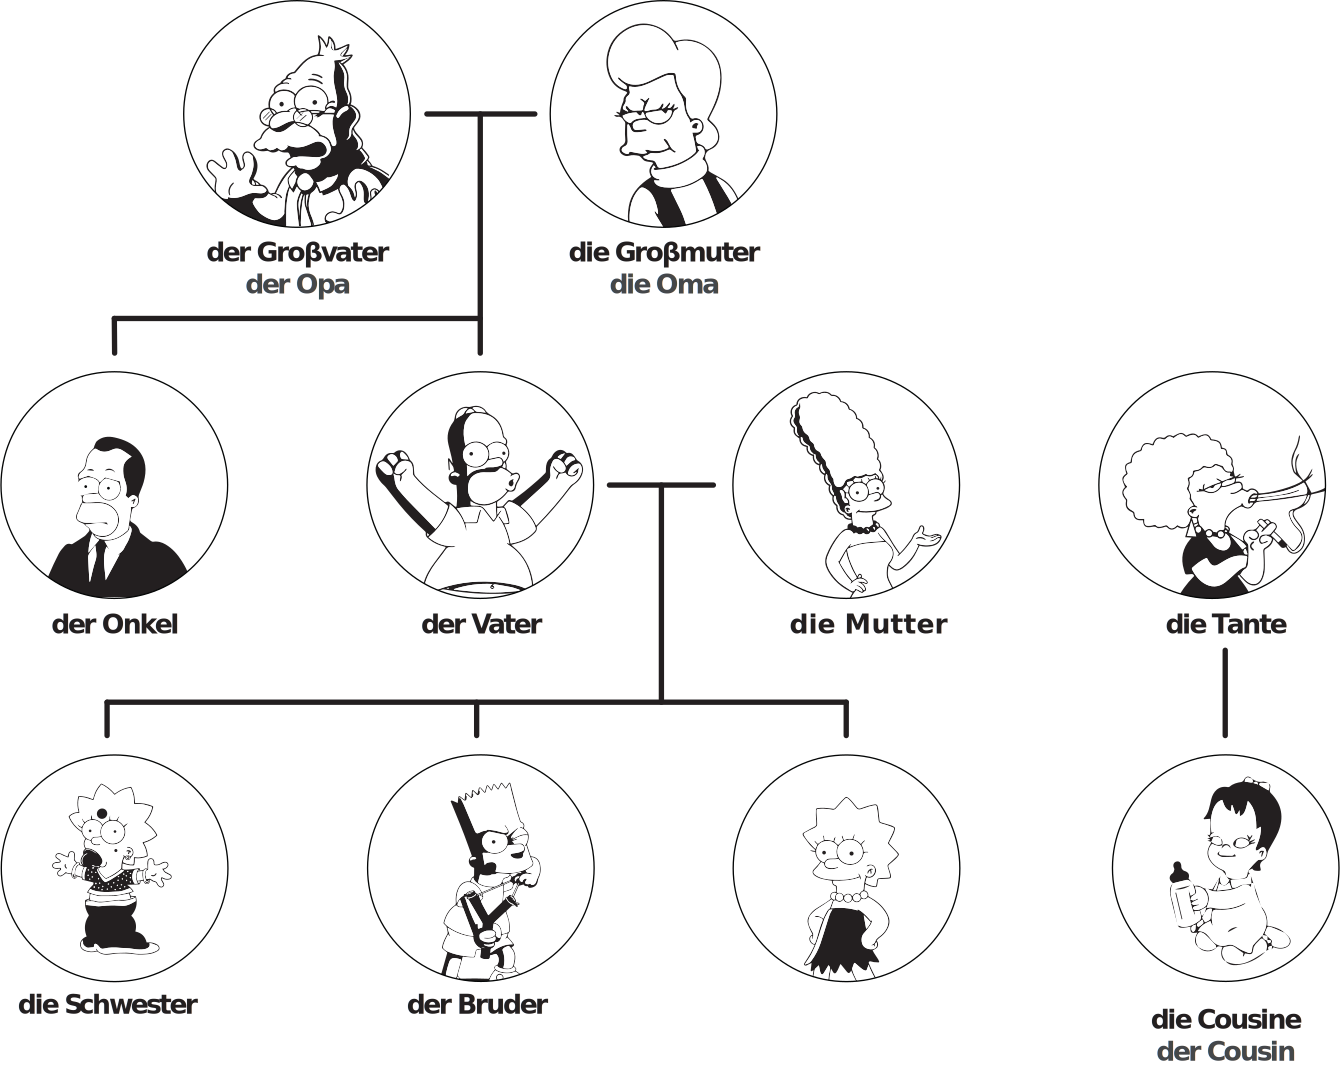
\includegraphics[width=.9\linewidth]{figures/family_tree.eps}

        \begin{longtabu}to \textwidth {>{\normalsize}X[1,m] >{\normalsize}X[1,m] >{\normalsize}X[1,m]}
            \toprule
            \textbf{Singular} & \textbf{Plural} & \textbf{Übersetzung} \\ 
            \toprule \endhead
                der Großvater/der Opa & die Großväter/die Opas & o avô\\ \hline
                der Großmutter/die Oma & die Großmütter/die Omas & a avó\\ \hline
                --- & die Großeltern & os avós\\ \hline
                der Enkel & die Enkel & o neto\\ \hline
                die Enkelin & die Enkelinnen & a neta\\ \hline
                --- & die Enkelkinder & os netos\\ \hline
                der Vater & die Väter & o pai\\ \hline
                die Mutter & die Mütter & a mãe\\ \hline
                --- & die Eltern & os pais\\ \hline
                der Sohn & die Söhne & o filho\\ \hline
                die Tochter & die Töchter & a filha\\ \hline
                --- & die Kinder & os filhos\\ \hline
                der Onkel & die Onkel & o tio\\ \hline
                die Tante & die Tanten & a tia\\ \hline
                der Cousin & die Cousins & o primo\\ \hline
                die Cousine & die Cousinen & a prima\\ \hline
                der Bruder & die Brüder & o irmão\\ \hline
                die Schwester & die Schwestern & a irmã\\ \hline
                --- & die Geschwister & os irmãos\\ \hline
            \toprule
        \end{longtabu}

        \subsection{Familiestand}\label{subsection:deutsch:familie:familiestand}

            \begin{itemize}[topsep=0pt,itemsep=4pt,parsep=0pt]
                \item[-] verheiratet \translation{casados}
                \item[-] geschieden \translation{separados}
                \item[-] zusammen \translation{juntos (namorados)}
                \item[-] getrennt \translation{separados (terminaram o namoro)}
                \item[-] single/ledig \translation{solteiro/solteira}
            \end{itemize}

    \vfill\null\pagebreak\section{der Termin / a marcação}\label{section:deutsch:der_termin}
    
        \subsection{die Uhrzeiten / o horário}\label{subsection:deutsch:die_uhrzeiten}

            \centering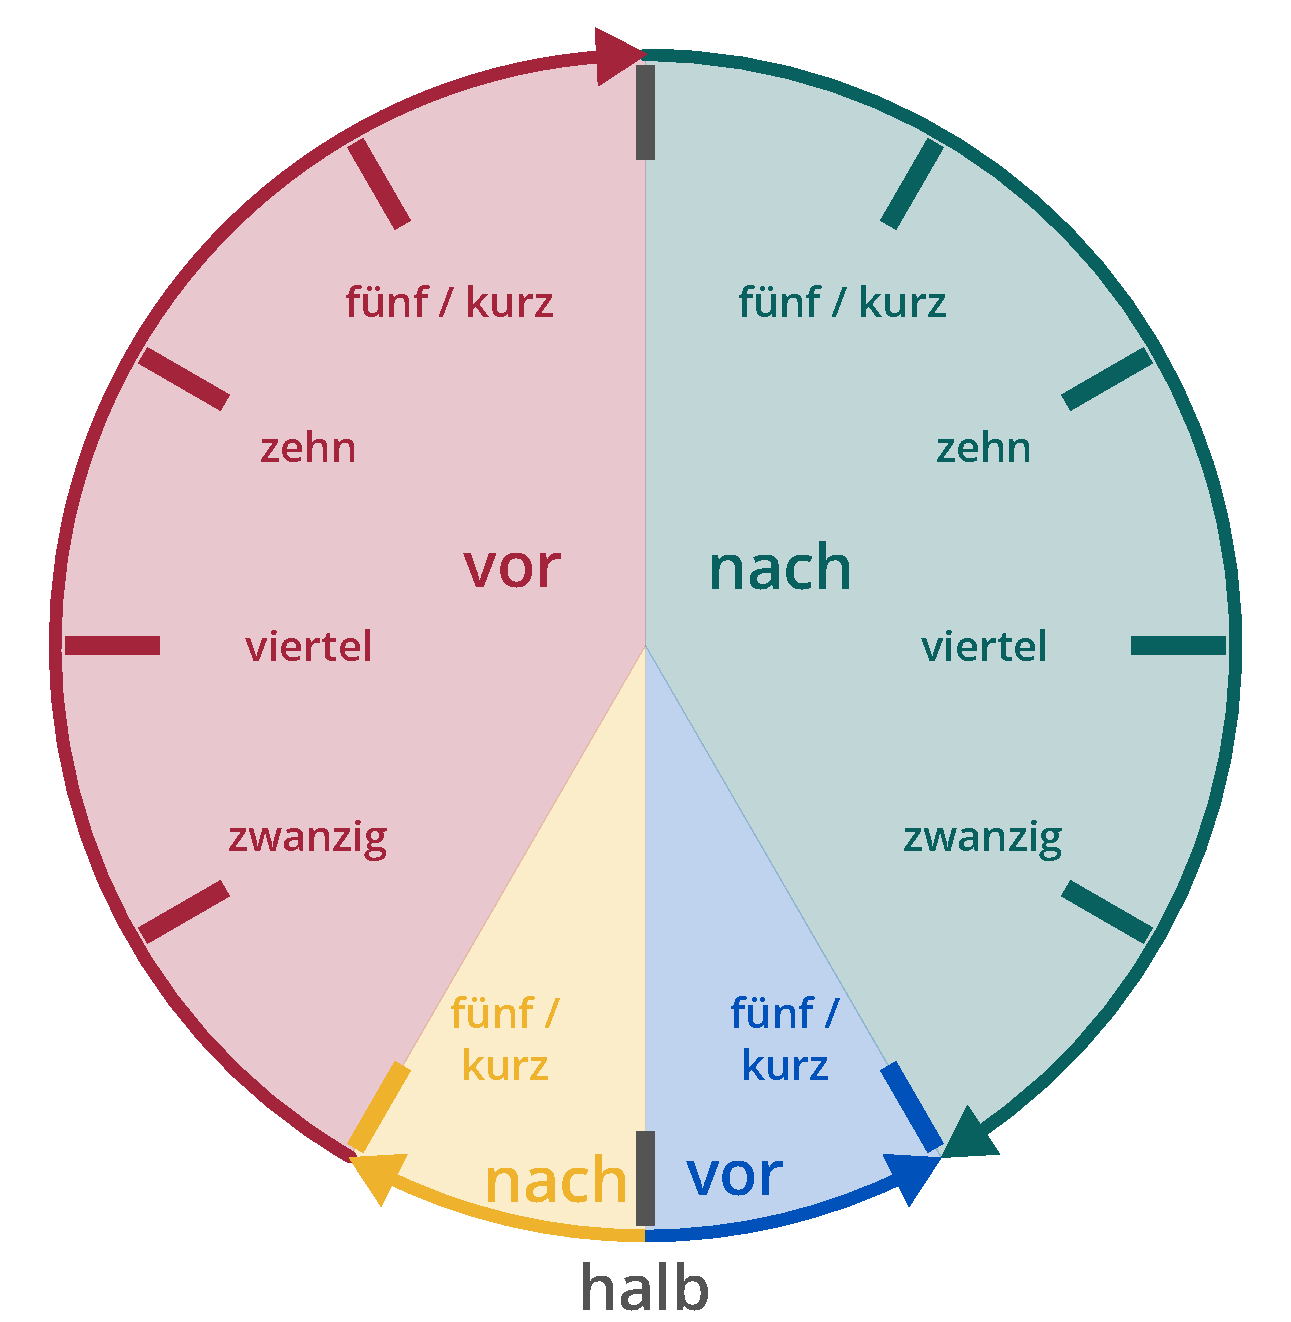
\includegraphics[width=.5\linewidth]{figures/uhrzeiten.pdf}

            \RaggedRight\textsb{Wie spät ist es? / Wie viel Uhr ist es?} \translation{Que horas são?}
            \begin{multicols}{2}
                \begin{itemize}[topsep=0pt,itemsep=4pt,parsep=0pt]
                    \item[] \textsb{18h}
                        \begin{itemize}
                            \item[-] Inoffizielle: Es ist (um/Punkt) sechs.
                            \item[-] Offizielle: Es ist achtzehn Uhr.
                        \end{itemize}
                    \item[] {\color{tropical_rain_forest}\textsb{15h05}}
                        \begin{itemize}
                            \item[-] Inoffizielle: {\color{tropical_rain_forest}Es ist  fünf/kurz nach drei.}
                            \item[-] Offizielle: {\color{tropical_rain_forest}Es ist fünfzehn Uhr fünf.}
                        \end{itemize}
                    \item[] {\color{absolute_zero}\textsb{16h25}}
                        \begin{itemize}
                            \item[-] Inoffizielle: {\color{absolute_zero}Es ist  fünf/kurz vor halb fünf.}
                            \item[-] Offizielle: {\color{absolute_zero}Es ist vierzehn Uhr fünfundzwanzig.}
                        \end{itemize}
                    \columnbreak
                    \item[] \textsb{17h30}
                        \begin{itemize}
                            \item[-] Inoffizielle: Es ist halb sechs.
                            \item[-] Offizielle: Es ist siebzehn Uhr dreißig.
                        \end{itemize}
                    \item[] {\color{saffron}\textsb{18h35}}
                        \begin{itemize}
                            \item[-] Inoffizielle: {\color{saffron}Es ist  fünf/kurz nach halb sieben.}
                            \item[-] Offizielle: {\color{saffron}Es ist achtzehn Uhr fünfunddreißig.}
                        \end{itemize}
                    \item[] {\color{deep_carmine}\textsb{19h45}}
                        \begin{itemize}
                            \item[-] Inoffizielle: {\color{deep_carmine}Es ist  viertel vor acht.}
                            \item[-] Offizielle: {\color{deep_carmine}Es ist siebzehn Uhr fünfundvierzig.}
                        \end{itemize}
                \end{itemize}
            \vfill\null
            \end{multicols}

    \subsection{die Wortstellung}\label{subsection:deutsch:wortstellung}

            \phonetics{Wortstellung}{vóót-xtélun}{posição frásica}
    
            \begin{multicols}{3}
                \raggedcolumns
                \subsubsection{der Hauptsatz}
    
                    \phonetics{Hauptsatz}{haupt-zatz}{oração principal}
    
                    
\includegraphics[width=.9\linewidth]{figures/dieHauptsatz.eps}
                    \label{fig:languages:deutsch:dieHauptsatz}
    
                \columnbreak
                \subsubsection{die Wortfrage oder W-Frage}
    
                    \phonetics{Wortfrage}{vóót-frrague}{pergunta}
    
                    
\includegraphics[width=.9\linewidth]{figures/dieWortfrage.eps}
                    \label{fig:languages:deutsch:dieWortfrage}
                \columnbreak
                \subsubsection{die Satzfrage oder Ja/Nein-Frage}
    
                    \phonetics{Satzfrage}{zats-frrague}{pergunta sim ou não}
    
                    
\includegraphics[width=.9\linewidth]{figures/dieSatzfrage.eps}
                    \label{fig:languages:deutsch:dieSatzfrage}
    
            \end{multicols}

    \subsection{Freunde, Kollegen und ich}\label{subsection:deutsch:freundekollegenich}

        \scriptsize
        \begin{longtabu}to \textwidth {X[1.2,m] | X[1,m] X[1,m] X[1,m] X[1,m] | X[1,m]}
            \toprule
            \multicolumn{6}{c}{\textbf{die} \phonetics{\textbf{Personen}}{pé-zou-nan}{pessoas}}\\
            \toprule
            \multirow{2}{*}{\textbf{die \phonetics{Übersetzung}{üba-ze-tzung}{tradução}}} & \multicolumn{4}{c|}{\textbf{Name}} & \multirow{2}{*}{\textbf{Adjektiv}} \\ 
            & \textsb{Mask. (der)} & \textsb{Fem. (die)} & \textsb{Neutrum (das)} & \textsb{Plural (die)} & \\ \tabucline-
                amiga & | & \phonetics{Freundin}{frróin-din}{} & | & \phonetics{Freundinen}{frróin-di-nan}{} & | \\ \hline
                amigo & \phonetics{Freund}{frróind}{} & | & | & \phonetics{Freunde}{frróin-da}{} & | \\ \hline
                (a) colega & | & \phonetics{Kollegin}{kó-lli-guin}{} & | & \phonetics{Kolleginen}{kó-lli-gui-nan}{} & | \\ \hline
                (o) colega & \phonetics{Kollege}{kó-lli-gue}{} & | & | & \phonetics{Kollegen}{kó-lli-gan}{} & | \\ \hline
                (a) companheira & | & \phonetics{Partnerin}{párr-tna-rrin}{} & | & \phonetics{Partnerinen}{párr-tna-rri-nan}{} & | \\ \hline
                (o) companheiro & \phonetics{Partner}{párr-tna}{} & | & | & \phonetics{Partner}{párr-tna}{} & | \\ \hline
                homem & \phonetics{Herr}{éarr}{} & | & | & \phonetics{Herren}{éa-rran}{} & | \\ \hline
                mulher & | & \phonetics{Frau}{frráu}{} & | & \phonetics{Frauen}{frráu-an}{} & | \\ \hline
                pessoa & | & \phonetics{Person}{pé-zoun}{} & | & \phonetics{Personen}{pé-zou-nan}{} & | \\ \hline
                pessoas & | & | & | & \phonetics{Leute}{llói-ta}{} & | \\ \hline
                ser humano & \phonetics{Mensch}{mén-x}{} & | & | & \phonetics{Menschen}{mén-xan}{} & | \\ \hline
        \end{longtabu}
        \normalsize

        \scriptsize
        \begin{longtabu}to \textwidth {X[1.2,m] | X[1,m] X[1,m] X[1,m] X[1,m] | X[1,m]}
            \toprule
            \multicolumn{6}{c}{\textbf{die} \phonetics{\textbf{Hobbys}}{hóbbis}{passatempos}}\\
            \toprule
            \multirow{2}{*}{\textbf{die \phonetics{Übersetzung}{üba-ze-tzung}{tradução}}} & \multicolumn{4}{c|}{\textbf{Name}} & \multirow{2}{*}{\textbf{Adjektiv}} \\ 
            & \textsb{Mask. (der)} & \textsb{Fem. (die)} & \textsb{Neutrum (das)} & \textsb{Plural (die)} & \\ \tabucline-
                favorito & \phonetics{Liebling}{lii-bling}{} & | & | & | & | \\ \hline
                fotografia & | & | & \phonetics{Foto}{fou-to}{} & \phonetics{Fotos}{fou-tos}{} & | \\ \hline
                livro & | & | & \phonetics{Buch}{burr}{} & \phonetics{Bücher}{bü-xa}{} & | \\ \hline
                música & | & \phonetics{Musik}{mu-zik}{} & | & | & | \\ \hline
                passatempo & | & | & \phonetics{Hobby}{hóbbi}{} & \phonetics{Hobbys}{hóbbis}{} & | \\ \hline
                tempo livre & | & \phonetics{Freizeit}{frrai-tssait}{} & | & | & | \\ \hline
        \end{longtabu}
        \normalsize

        \scriptsize
        \begin{longtabu}to \textwidth {X[1.2,m] | X[1,m] X[1,m] X[1,m] X[1,m] | X[1,m]}
            \toprule
            \multicolumn{6}{c}{\textbf{der} \phonetics{\textbf{Freizeit}}{frrai-tssait}{tempo livre}}\\
            \toprule
            \multirow{2}{*}{\textbf{die \phonetics{Übersetzung}{üba-ze-tzung}{tradução}}} & \multicolumn{4}{c|}{\textbf{Name}} & \multirow{2}{*}{\textbf{Adjektiv}} \\ 
            & \textsb{Mask. (der)} & \textsb{Fem. (die)} & \textsb{Neutrum (das)} & \textsb{Plural (die)} & \\ \tabucline-
                café & | & | & \phonetics{Café}{ká-fê}{} & \phonetics{Cafés}{ká-fês}{} & | \\ \hline
                cinema & | & | & \phonetics{Kino}{kí-nou}{} & \phonetics{Kinos}{kí-nous}{} & | \\ \hline
                estádio de futebol & | & | & \phonetics{Fußballstadion}{fuss-báll-xtádium}{} & \phonetics{Fußballstadien}{fuss-báll-xtádian}{} & | \\ \hline
                museu & | & | & \phonetics{Museum}{mu-zê-um}{} & \phonetics{Museen}{mu-ziin}{} & | \\ \hline
                piscina & | & | & \phonetics{Schwimmbad}{xvim-bád}{} & \phonetics{Schwimmbäder}{xvim-béda}{} & | \\ \hline
                teatro & | & | & \phonetics{Theater}{tê-à-ta}{} & \phonetics{Theater}{tê-à-ta}{} & | \\ \hline
        \end{longtabu}
        \normalsize

        \scriptsize
        \begin{longtabu}to \textwidth {X[1.2,m] | X[1,m] X[1,m] X[1,m] X[1,m] | X[1,m]}
            \toprule
            \multicolumn{6}{c}{\textbf{die} \phonetics{\textbf{Berufe}}{béa-rru-fa}{profissões}}\\
            \toprule
            \multirow{2}{*}{\textbf{die \phonetics{Übersetzung}{üba-ze-tzung}{tradução}}} & \multicolumn{4}{c|}{\textbf{Name}} & \multirow{2}{*}{\textbf{Adjektiv}} \\ 
            & \textsb{Mask. (der)} & \textsb{Fem. (die)} & \textsb{Neutrum (das)} & \textsb{Plural (die)} & \\ \tabucline-
                arquitecta & | & \phonetics{Architektin}{àrr-xi-ték-tin}{} & | & \phonetics{Architektinen}{àrr-xi-ték-ti-nan}{} & | \\ \hline
                arquitecto & \phonetics{Architekt}{àrr-xi-tékt}{} & | & | & \phonetics{Architekten}{àrr-xi-ték-tan}{} & | \\ \hline
                cozinheira & | & \phonetics{Köchin}{kö-rrin}{} & | & \phonetics{Köchinnen}{kö-rri-nan}{} & | \\ \hline
                cozinheiro & \phonetics{Koch}{kórr}{} & | & | & \phonetics{Köche}{kö-rra}{} & | \\ \hline
                empresa & | & \phonetics{Firma}{fêrr-ma}{} & | & \phonetics{Firmen}{fêrr-man}{} & | \\ \hline
                engenheira & | & \phonetics{Ingenieurin}{en-ge-niaa-rrin}{} & | & \phonetics{Ingenieurinnen}{en-ge-niaa-rri-nan}{} & | \\ \hline
                engenheiro & \phonetics{Ingenieur}{en-ge-niaa}{} & | & | & \phonetics{Ingenieure}{en-ge-niaa-rra}{} & | \\ \hline
                (a) estudante (uni) & | & \phonetics{Studentin}{xtu-den-tin}{} & | & \phonetics{Studentinnen}{xtu-den-ti-nan}{} & | \\ \hline
                (o) estudante (uni) & \phonetics{Student}{xtu-den-te}{} & | & | & \phonetics{Studenten}{xtu-den-tan}{} & | \\ \hline
                (a) jornalista & | & \phonetics{Journalistin}{jourr-na-lis-tin}{} & | & \phonetics{Journalistinnen}{jourr-na-lis-ti-nan}{} & | \\ \hline
                (o) jornalista & \phonetics{Journalist}{jourr-na-list}{} & | & | & \phonetics{Journalisten}{jourr-na-lis-tan}{} & | \\ \hline
                médica & | & \phonetics{Ärztin}{érr-tstin}{} & | & \phonetics{Ärztinen}{érr-tsti-nan}{} & | \\ \hline
                médico & \phonetics{Arzt}{àrr-tst}{} & | & | & \phonetics{Ärzte}{érr-tsta}{} & | \\ \hline
                profesora (uni) & | & \phonetics{Professorin}{prrou-fé-ssou-rrin}{} & | & \phonetics{Professorinnen}{prrou-fé-ssou-rri-nan}{} & | \\ \hline
                professor (uni) & \phonetics{Professor}{prrou-fé-ssoua}{} & | & | & \phonetics{Professoren}{prrou-fé-ssou-rran}{} & | \\ \hline
                profissão & \phonetics{Beruf}{béa-rruf}{} & | & | & \phonetics{Berufe}{béa-rru-fa}{} & | \\ \hline
                (a) pugilista & | & \phonetics{Boxerin}{bó-kssa-rrin}{} & | & \phonetics{Boxerinnen}{bó-kssa-rri-nan}{} & | \\ \hline
                (o) pugilista & \phonetics{Boxer}{bó-kssa}{} & | & | & \phonetics{Boxer}{bó-kssa}{} & | \\ \hline
                (a) taxista & | & \phonetics{Taxifahrerin}{tá-cssi-fá-rra-rrin}{} & | & \phonetics{Taxifahrerinnen}{tá-cssi-fá-rra-rri-nan}{} & | \\ \hline
                (o) taxista & \phonetics{Taxifahrer}{tá-cssi-fá-rrá}{} & | & | & \phonetics{Taxifahrer}{tá-cssi-fá-rrá}{} & | \\ \hline
                técnica & | & \phonetics{Technikerin}{téx-ni-ca-rrin}{} & | & \phonetics{Technikerinnen}{téx-ni-ca-rri-nan}{} & | \\ \hline
                técnico & \phonetics{Techniker}{téx-ni-ca}{} & | & | & \phonetics{Techniker}{téx-ni-ca}{} & | \\ \hline
        \end{longtabu}
        \normalsize

    \subsection{in der Stadt}\label{subsection:deutsch:stadt}

        \scriptsize
        \begin{longtabu}to \textwidth {X[1.2,m] | X[1,m] X[1,m] X[1,m] X[1,m] | X[1,m]}
            \toprule
            \multicolumn{6}{c}{\textbf{mit} \phonetics{\textbf{Verkehrsmitteln}}{rés-to-rran}{meios de transporte} \phonetics{\textbf{unterwegs}}{rés-to-rran}{a caminho}}\\
            \toprule
            \multirow{2}{*}{\textbf{die \phonetics{Übersetzung}{üba-ze-tzung}{tradução}}} & \multicolumn{4}{c|}{\textbf{Name}} & \multirow{2}{*}{\textbf{Adjektiv}} \\ 
            & \textsb{Mask. (der)} & \textsb{Fem. (die)} & \textsb{Neutrum (das)} & \textsb{Plural (die)} & \\ \tabucline-
                autocarro & \phonetics{Bus}{bouss}{} & | & | & \phonetics{Busse}{bou-ssa}{} & | \\ \hline
                avião & | & | & \phonetics{Flugzeug}{fllug-tssóig}{} & \phonetics{Flugzeuge}{fllug-tssói-ga}{} & | \\ \hline
                barco & | & | & \phonetics{Schiff}{xêf}{} & \phonetics{Schiffe}{xê-fa}{} & | \\ \hline
                bicicleta & | & | & \phonetics{Fahrrad}{fá-rrád}{} & \phonetics{Fahrräder}{fá-rré-da}{} & | \\ \hline
                bilhete & | & | & \phonetics{Ticket}{ti-cat}{} & \phonetics{Tickets}{ti-cats}{} & | \\ \hline
                bilhete de viagem & | & \phonetics{Fahrkarte}{fá-karr-ta}{} & | & \phonetics{Fahrkarten}{fá-karr-tan}{} & | \\ \hline
                comboio & \phonetics{Zug}{tssug}{} & | & | & \phonetics{Züge}{tssü-ga}{} & | \\ \hline
                eléctrico & | & \phonetics{Straßenbahn}{xtrrá-ssan-bán}{} & | & \phonetics{Straßenbahnen}{xtrrá-ssan-bá-nan}{} & | \\ \hline
                meio de transporte & | & | & \phonetics{Verkehrsmittel}{fa-kêa-ssmi-tall}{} & \phonetics{Verkehrsmitteln}{fa-kêa-ssmi-talln}{} & | \\ \hline
                metro & | & \phonetics{U-Bahn}{u-bán}{} & | & \phonetics{U-Bahnen}{u-bá-nan}{} & | \\ \hline
                metro de superfície & | & \phonetics{S-Bahn}{ésse-bán}{} & | & \phonetics{S-Bahnen}{ésse-bá-nan}{} & | \\ \hline
                passageiro & \phonetics{Passagier}{pá-ssá-gia}{} & | & | & \phonetics{Passagiere}{pá-ssá-gii-rra}{} & | \\ \hline
        \end{longtabu}
        \normalsize

        \scriptsize
        \begin{longtabu}to \textwidth {X[1.2,m] | X[1,m] X[1,m] X[1,m] X[1,m] | X[1,m]}
            \toprule
            \multicolumn{6}{c}{\phonetics{\textbf{Orte}}{óór-ta}{locais}}\\
            \toprule
            \multirow{2}{*}{\textbf{die \phonetics{Übersetzung}{üba-ze-tzung}{tradução}}} & \multicolumn{4}{c|}{\textbf{Name}} & \multirow{2}{*}{\textbf{Adjektiv}} \\ 
            & \textsb{Mask. (der)} & \textsb{Fem. (die)} & \textsb{Neutrum (das)} & \textsb{Plural (die)} & \\ \tabucline-
                aeroporto & \phonetics{Flughafen}{fllug-há-fan}{} & | & | &  \phonetics{Flughäfen}{fllug-hé-fan}{} & | \\ \hline
                câmara municipal & | & | & \phonetics{Rathaus}{rát-hauss}{} & \phonetics{Rathäuser}{rát-hoi-za}{} & | \\ \hline
                caminho & \phonetics{Weg}{vig}{} & | & | & \phonetics{Wege}{vii-ga}{} & | \\ \hline
                cidade & | & \phonetics{Stadt}{xtá-t}{} & | & \phonetics{Städte}{xté-te}{} & | \\ \hline
                estação de comboios & \phonetics{Bahnhof}{bán-hóf}{} & | & | &  \phonetics{Bahnhöfe}{bán-hafa}{} & | \\ \hline
                igreja & | & \phonetics{Kirche}{kirr-xa}{} & | & \phonetics{Kirchen}{kirr-xan}{} & | \\ \hline
                hotel & | & | & \phonetics{Hotel}{hou-tell}{} & \phonetics{Hotels}{hou-tells}{} & | \\ \hline
                lago & \phonetics{See}{zii}{} & | & | &  \phonetics{Seen}{ziin}{} & | \\ \hline
                local & \phonetics{Ort}{óort}{} & | & | &  \phonetics{Orte}{óor-ta}{} & | \\ \hline
                loja & | & | & \phonetics{Geschäft}{ga-xéft}{} & \phonetics{Geschäfte}{ga-xéf-ta}{} & | \\ \hline
                mar & | & | & \phonetics{Meer}{mêa}{} & \phonetics{Meere}{mêa-rra}{} & | \\ \hline
                mercado & \phonetics{Markt}{márr-kt}{} & | & | & \phonetics{Märkte}{mérr-kta}{} & | \\ \hline
                parque & \phonetics{Park}{pá-k}{} & | & | & \phonetics{Park}{pá-ks}{} & | \\ \hline
                porto & \phonetics{Hafen}{há-fan}{} & | & | &  \phonetics{Häfen}{hé-fan}{} & | \\ \hline
                rio & \phonetics{Fluss}{flo-ss}{} & | & | &  \phonetics{Flüsse}{flü-ssa}{} & | \\ \hline
                rua & | & \phonetics{Straße}{xtrrá-ssa}{} & | & \phonetics{Straßen}{xtrrá-ssan}{} & | \\ \hline
                terminal & \phonetics{Terminal}{térr-mi-náll}{} & | & | &  \phonetics{Terminals}{térr-mi-nálls}{} & | \\ \hline
                torre & \phonetics{Turm}{toum}{} & | & | & \phonetics{Türme}{tür-ma}{} & | \\ \hline
        \end{longtabu}
        \normalsize

        \scriptsize
        \begin{longtabu}to \textwidth {X[1.2,m] | X[1,m] X[1,m] X[1,m] X[1,m] | X[1,m]}
            \toprule
            \multicolumn{6}{c}{\phonetics{\textbf{Orientierung}}{ó-rrien-tii-run}{orientação}}\\
            \toprule
            \multirow{2}{*}{\textbf{die \phonetics{Übersetzung}{üba-ze-tzung}{tradução}}} & \multicolumn{4}{c|}{\textbf{Name}} & \multirow{2}{*}{\textbf{Adjektiv}/\textbf{Adverb}} \\ 
            & \textsb{Mask. (der)} & \textsb{Fem. (die)} & \textsb{Neutrum (das)} & \textsb{Plural (die)} & \\ \tabucline-
                alto & | & | & | & | & \phonetics{hoch}{ou-rr}{} \\ \hline
                bonito & | & | & | & | & \phonetics{schön}{xoun}{} \\ \hline
                comprido & | & | & | & | & \phonetics{lang}{llang}{} \\ \hline
                curto & | & | & | & | & \phonetics{kurz}{kourr-ts}{} \\ \hline
                direita & | & | & | & | & \phonetics{rechts}{réchh-tss}{} \\ \hline
                em frente & | & | & | & | & \phonetics{geradeaus}{ga-rráde-auz}{} \\ \hline
                esquerda & | & | & | & | & \phonetics{links}{llink-ss}{} \\ \hline
                fácil & | & | & | & | & \phonetics{einfach}{aine-fárr}{} \\ \hline
                grande & | & | & | & | & \phonetics{groß}{grrou-ss}{} \\ \hline
                idade & | & | & | & | & \phonetics{alt}{à-llt}{} \\ \hline
                largo & | & | & | & | & \phonetics{breit}{brrait}{} \\ \hline
                metro & \phonetics{Meter}{mé-ta}{} & | & | & \phonetics{Meter}{mé-ta}{} & | \\ \hline
                moderno & | & | & | & | & \phonetics{modern}{mou-derrn}{} \\ \hline
                plano & \phonetics{Plan}{plá-n}{} & | & | & \phonetics{Pläne}{plé-na}{} & | \\ \hline
                sempre & | & | & | & | & \phonetics{immer}{ima}{} \\ \hline
                todo(s) & | & | & | & | & \phonetics{alle}{à-lle}{} \\ \hline
        \end{longtabu}
        \normalsize

        \scriptsize
        \begin{longtabu}to \textwidth {X[1.2,m] | X[1,m] X[1,m] X[1,m] X[1,m] | X[1,m]}
            \toprule
            \multicolumn{6}{c}{\phonetics{\textbf{Veranstaltungen}}{fa-àn-xtáll-tun-gan}{eventos}}\\
            \toprule
            \multirow{2}{*}{\textbf{die \phonetics{Übersetzung}{üba-ze-tzung}{tradução}}} & \multicolumn{4}{c|}{\textbf{Name}} & \multirow{2}{*}{\textbf{Adjektiv}/\textbf{Adverb}} \\ 
            & \textsb{Mask. (der)} & \textsb{Fem. (die)} & \textsb{Neutrum (das)} & \textsb{Plural (die)} & \\ \tabucline-
                concerto & | & | & \phonetics{Konzert}{coun-tssérrt}{} & \phonetics{Konzerte}{coun-tssérr-ta}{} & | \\ \hline
                evento & | & \phonetics{Veranstaltung}{fa-àn-xtáll-tun}{} & | & \phonetics{Veranstaltungen}{fa-àn-xtáll-tun-gan}{} & | \\ \hline
                evento & \phonetics{Event}{i-vent}{} & | & | & \phonetics{Events}{i-vents}{} & | \\ \hline
                festival & | & | & \phonetics{Festival}{fés-ti-vell}{} & \phonetics{Festivals}{fés-ti-vells}{} & | \\ \hline
                filme & \phonetics{Film}{fill-m}{} & | & | & \phonetics{Filme}{fill-ma}{} & | \\ \hline
                orquestra & | & | & \phonetics{Orchester}{ó-kés-ta}{} & \phonetics{Orchester}{ó-kés-ta}{} & | \\ \hline
        \end{longtabu}
        \normalsize

        \scriptsize
        \begin{longtabu}to \textwidth {X[1.2,m] | X[1,m] X[1,m] X[1,m] X[1,m] | X[1,m]}
            \toprule
            \multicolumn{6}{c}{\textbf{Andere}}\\
            \toprule
            \multirow{2}{*}{\textbf{die \phonetics{Übersetzung}{üba-ze-tzung}{tradução}}} & \multicolumn{4}{c|}{\textbf{Name}} & \multirow{2}{*}{\textbf{Adjektiv}/\textbf{Adverb}} \\ 
            & \textsb{Mask. (der)} & \textsb{Fem. (die)} & \textsb{Neutrum (das)} & \textsb{Plural (die)} & \\ \tabucline-
                teste/prova & \phonetics{Test}{tésst}{} & | & | & \phonetics{Tests}{téss-ts}{} & | \\ \hline
                (o) visitante & \phonetics{Besucher}{ba-zu-rra}{} & | & | & \phonetics{Besucher}{ba-zu-rra}{} & | \\ \hline
        \end{longtabu}
        \normalsize

    \subsection{Das Familie}\label{subsection:deutsch:familie}

        \begin{itemize}
            \item[der \phonetics{Familienstand}{fá-mí-llian-xtand}{estado civil}] \phonetics{Sind}{zind}{é} \phonetics{Sie}{zii}{você} \phonetics{ledig}{li-dichh}{solteiro}? $\rightarrow$ \textit{É solteiro?}
        \end{itemize}

        \scriptsize
        \begin{longtabu}to \textwidth {X[1.2,m] | X[1,m] X[1,m] X[1,m] X[1,m] | X[1,m]}
            \toprule
            \multicolumn{6}{c}{\textbf{die} \phonetics{\textbf{Verwandten}}{fé-rran-tan}{}}\\
            \toprule
            \multirow{2}{*}{\textbf{die \phonetics{Übersetzung}{üba-ze-tzung}{tradução}}} & \multicolumn{4}{c|}{\textbf{Name}} & \multirow{2}{*}{\textbf{Adjektiv}} \\ 
            & \textsb{Mask. (der)} & \textsb{Fem. (die)} & \textsb{Neutrum (das)} & \textsb{Plural (die)} & \\ \tabucline-
                avó & | & \phonetics{Großmutter}{grróuss-mu-ta}{}/\phonetics{Oma}{Ou-má}{} & | & \phonetics{Großmütter}{grróuss-mü-ta}{}/\phonetics{Omas}{Ou-más}{} & | \\ \hline
                avô & \phonetics{Großvater}{grróuss-fá-ta}{}/\phonetics{Opa}{Ou-pá}{} & | & | & \phonetics{Großväter}{grróuss-fé-ta}{}/\phonetics{Opas}{Ou-pás}{} & | \\ \hline
                avós & | & | & | & \phonetics{Großeltern}{grróuss-éll-tan}{} & | \\ \hline
                bebé & | & | & \phonetics{Baby}{bei-bi}{} & \phonetics{Babys}{bei-bis}{} & | \\ \hline
                casal & \phonetics{Ehepartner}{êê-part-na}{} & | & | & \phonetics{Ehepartner}{êê-part-na}{} & | \\ \hline
                criança & | & | & \phonetics{Kind}{kind}{} & \phonetics{Kinder}{kin-da}{} & | \\ \hline
                cunhada & \phonetics{Schwägerin}{xvé-ga-rrin}{} & | & | & \phonetics{Schwägerinnen}{xvé-ga-rri-nan}{} & | \\ \hline
                cunhado & \phonetics{Schwager}{xvá-ga}{} & | & | & \phonetics{Schwäger}{xvé-ga}{} & | \\ \hline
                esposa & | & \phonetics{Ehefrau}{êê-frrau}{} & | & \phonetics{Ehefrauen}{êê-frrauan}{} & | \\ \hline
                esposo & \phonetics{Ehemann}{êê-mán}{} & | & | & \phonetics{Ehemänner}{êê-mé-na}{} & | \\ \hline
                familiar & \phonetics{Verwandte}{fé-rran-ta}{} & \phonetics{Verwandte}{fé-rran-ta}{} & | & \phonetics{Verwandten}{fé-rran-tan}{} & | \\ \hline
                filha & \phonetics{Tochter}{tórr-ta}{} & | & | & \phonetics{Tochter}{törr-ta}{} & | \\ \hline
                filho & \phonetics{Sohn}{zou-n}{} & | & | & \phonetics{Söhne}{zö-na}{} & | \\ \hline
                irmã & | & \phonetics{Schwester}{xvés-ta}{} & | & \phonetics{Schwestern}{xvés-tan}{} & | \\ \hline
                irmão & \phonetics{Bruder}{brru-da}{} & | & | & \phonetics{Brüder}{brrü-da}{} & | \\ \hline
                irmãos & | & | & | & \phonetics{Geschwister}{ga-xvis-ta}{} & | \\ \hline
                mãe & | & \phonetics{Mutter}{mu-ta}{} & | & \phonetics{Mütter}{mü-ta}{} & | \\ \hline
                pai & \phonetics{Vater}{fá-ta}{} & | & | & \phonetics{Väter}{fé-ta}{} & | \\ \hline
                pais & | & | & | & \phonetics{Eltern}{éll-tan}{} & | \\ \hline
                prima & | & \phonetics{Kusine}{cu-zi-na}{} & | &  & | \\ \hline
                primo & \phonetics{Cousin}{cou-zan}{} & | & | & \phonetics{Cousins}{cou-zans}{} & | \\ \hline
                sobrinha & \phonetics{Nichte}{nich-ta}{} & | & | & \phonetics{Nichten}{nich-tan}{} & | \\ \hline
                sobrinho & \phonetics{Neffe}{né-fa}{} & | & | & \phonetics{Neffen}{né-fan}{} & | \\ \hline
                tia & | & \phonetics{Tante}{tán-ta}{} & | & \phonetics{Tanten}{tán-tan}{} & | \\ \hline
                tio & \phonetics{Onkel}{on-kall}{} & | & | & \phonetics{Onkel}{on-kall}{} & | \\ \hline
        \end{longtabu}
        \normalsize

        \scriptsize
        \begin{longtabu}to \textwidth {X[1.2,m] | X[1,m] X[1,m] X[1,m] X[1,m] | X[1,m]}
            \multirow{2}{*}{\textbf{die \phonetics{Übersetzung}{üba-ze-tzung}{tradução}}} & \multicolumn{4}{c|}{\textbf{Name}} & \multirow{2}{*}{\textbf{Adjektiv}} \\ 
             & \textsb{Mask. (der)} & \textsb{Fem. (die)} & \textsb{Neutrum (das)} & \textsb{Plural (die)} & \\ \tabucline-
                casado & | & | & | & | & \phonetics{verheiratet}{fa-rrai-rra-tat}{}\\ \hline
                divorciado & | & | & | & | & \phonetics{geschieden}{ga-xii-dan}{}\\ \hline
                solteiro & | & | & | & | & \phonetics{ledig}{li-dichh}{} \phonetics{single}{zin-gal}{} \\ \hline
        \end{longtabu}
        \normalsize

    \subsection{Lebensmittel}\label{subsection:deutsch:lebensmittel}

        \scriptsize
        \begin{longtabu}to \textwidth {X[1.2,m] | X[1,m] X[1,m] X[1,m] X[1,m] | X[1,m]}
            \toprule
            \multicolumn{6}{c}{\textbf{das Obst}}\\
            \toprule
            \multirow{2}{*}{\textbf{die \phonetics{Übersetzung}{üba-ze-tzung}{tradução}}} & \multicolumn{4}{c|}{\textbf{Name}} & \multirow{2}{*}{\textbf{Adjektiv}} \\ 
            & \textsb{Mask. (der)} & \textsb{Fem. (die)} & \textsb{Neutrum (das)} & \textsb{Plural (die)} & \\ \tabucline-
                ameixa & | & \phonetics{Pflaume}{pfllau-ma}{} & | & \phonetics{Pflaumen}{pfllau-man}{} & | \\ \hline
                ananás & | & \phonetics{Ananas}{à-na-náss}{} & | & \phonetics{Ananasse}{à-na-ná-ssa}{} & | \\ \hline
                banana & | & \phonetics{Banane}{bá-ná-ne}{} & | & \phonetics{Bananen}{bá-ná-nan}{} & | \\ \hline
                cereja & | & \phonetics{Kirsche}{quirr-xe}{} & | & \phonetics{Kirschen}{quirr-xan}{} & | \\ \hline
                kiwi & | & \phonetics{Kiwi}{kí-vi}{} & | & \phonetics{Kiwis}{kí-viss}{} & | \\ \hline
                laranja & | & \phonetics{Orange}{ó-rran-ja}{} & | & \phonetics{Orangen}{ó-rran-jan}{} & | \\ \hline
                limão & | & \phonetics{Zitrone}{tzi-trró-na}{} & | & \phonetics{Zitronen}{tzi-trró-nan}{} & | \\ \hline
                maçã & \phonetics{Apfel}{à-pfall}{} & | & | & \phonetics{Äpfel}{é-pfall}{} & | \\ \hline
                mango & | & \phonetics{Mango}{mãn-gou}{} & | & \phonetics{Mangos}{mãn-gouss}{} & | \\ \hline
                melancia & | & \phonetics{Wassermelone}{vá-ssa-mê-llou-na}{} & | & \phonetics{Wassermelonen}{vá-ssa-mê-llou-nan}{} & | \\ \hline
                melão & | & \phonetics{Melone}{mê-llou-na}{} & | & \phonetics{Melonen}{mê-llou-nan}{} & | \\ \hline
                morango & | & \phonetics{Erdbeere}{érr-birre}{} & | & \phonetics{Erdbeeren}{érr-birran}{} & | \\ \hline
                pêra & | & \phonetics{Birne}{birr-na}{} & | & \phonetics{Birnen}{birr-nan}{} & | \\ \hline
                tomate & | & \phonetics{Tomate}{tó-má-te}{} & | & \phonetics{Tomaten}{tó-má-tan}{} & | \\ \hline
                uva & | & \phonetics{Traube}{trráu-be}{} & | & \phonetics{Trauben}{trráu-ban}{} & | \\ \hline
        \end{longtabu}
        \normalsize

        \scriptsize
        \begin{longtabu}to \textwidth {X[1.2,m] | X[1,m] X[1,m] X[1,m] X[1,m] | X[1,m]}
            \toprule
            \multicolumn{6}{c}{\textbf{das Gemüse}}\\
            \toprule
            \multirow{2}{*}{\textbf{die \phonetics{Übersetzung}{üba-ze-tzung}{tradução}}} & \multicolumn{4}{c|}{\textbf{Name}} & \multirow{2}{*}{\textbf{Adjektiv}} \\ 
            & \textsb{Mask. (der)} & \textsb{Fem. (die)} & \textsb{Neutrum (das)} & \textsb{Plural (die)} & \\ \tabucline-
                alface & \phonetics{(Kopf)salat}{(cópf-)zá-llá-t}{} & | & | & \phonetics{(Kopf)salate}{(cópf-)zá-llá-ta}{} & | \\ \hline
                alho & \phonetics{Knoblauch}{cnoub-llaurr}{} & | & | & \phonetics{Knoblauch}{cnoub-llaurr}{} & | \\ \hline
                azeite & | & | & \phonetics{Olivenöl}{ou-lívan-öll}{} & | & | \\ \hline
                azeitona & \phonetics{Olive}{ou-lí-va}{} & | & | & \phonetics{Oliven}{ou-lí-van}{} & | \\ \hline
                cebola & | & \phonetics{Zwiebel}{tsvi-ball}{} & | & \phonetics{Zwiebeln}{tsvi-balln}{} & | \\ \hline
                cenoura & | & \phonetics{Möhre}{mö-rra}{}/\phonetics{Karotte}{ká-rró-ta}{} & | & \phonetics{Möhren}{mö-rran}{}/\phonetics{Karotte}{ká-rró-tan}{} & | \\ \hline
                couve & \phonetics{Kohl}{cou-ll}{} & | & | & \phonetics{Kohle}{cou-lla}{} & | \\ \hline
                batata & | & \phonetics{Kartoffel}{kar-tó-fall}{} & | & \phonetics{Kartoffeln}{kar-tó-falln}{} & | \\ \hline
                pepino & | & \phonetics{Gurke}{gurr-ka}{} & | & \phonetics{Gurken}{gurr-kan}{} & | \\ \hline
                pimenta & \phonetics{Pfeffer}{pfé-fa}{} & | & | & \phonetics{Pfeffer}{pfé-fa}{} & | \\ \hline
                pimento/paprica & \phonetics{Paprika}{pá-prri-cá}{} & | & | & \phonetics{Paprika}{pá-prri-cá}{} & | \\ \hline
        \end{longtabu}
        \normalsize

        \scriptsize
        \begin{longtabu}to \textwidth {X[1.2,m] | X[1,m] X[1,m] X[1,m] X[1,m] | X[1,m]}
            \toprule
            \multicolumn{6}{c}{\textbf{die} \phonetics{\textbf{Milchprodukte}}{millxe-prro-dukta}{derivados do leite}}\\
            \toprule
            \multirow{2}{*}{\textbf{die \phonetics{Übersetzung}{üba-ze-tzung}{tradução}}} & \multicolumn{4}{c|}{\textbf{Name}} & \multirow{2}{*}{\textbf{Adjektiv}} \\ 
            & \textsb{Mask. (der)} & \textsb{Fem. (die)} & \textsb{Neutrum (das)} & \textsb{Plural (die)} & \\ \tabucline-
                iogurte & \phonetics{Joghurt}{ió-górr-t}{} & | & | & \phonetics{Joghurts}{ió-górr-ts}{} & | \\ \hline
                manteiga & | & \phonetics{Butter}{bu-ta}{} & | & \phonetics{Butter}{bu-ta}{} & | \\ \hline
                natas & | & \phonetics{Sahne}{zá-ne}{} & | & \phonetics{Sahne}{zá-ne}{} & | \\ \hline
                queijo & \phonetics{Käse}{que-ze}{} & | & | & \phonetics{Käse}{que-ze}{} & | \\ \hline
        \end{longtabu}
        \normalsize

        \scriptsize
        \begin{longtabu}to \textwidth {X[1.2,m] | X[1,m] X[1,m] X[1,m] X[1,m] | X[1,m]}
            \toprule
            \multicolumn{6}{c}{\textbf{die} \phonetics{\textbf{Backwaren}}{báque-va-rran}{pastelaria}}\\
            \toprule
            \multirow{2}{*}{\textbf{die \phonetics{Übersetzung}{üba-ze-tzung}{tradução}}} & \multicolumn{4}{c|}{\textbf{Name}} & \multirow{2}{*}{\textbf{Adjektiv}} \\ 
            & \textsb{Mask. (der)} & \textsb{Fem. (die)} & \textsb{Neutrum (das)} & \textsb{Plural (die)} & \\ \tabucline-
                bolacha & \phonetics{Keks}{kê-kss}{} & | & | & \phonetics{Kekse}{kê-kza}{} & | \\ \hline
                bolo & \phonetics{Kuchen}{cu-rran}{} & | & | & \phonetics{Kuchen}{cu-rran}{} & | \\ \hline
                pão & | & | & \phonetics{Brot}{brrou-t}{} & \phonetics{Brote}{brrou-ta}{} & | \\ \hline
                papo-seco & | & | & \phonetics{Brötchen}{brrou-txan}{} & \phonetics{Brötchen}{brrou-txan}{} & | \\ \hline
        \end{longtabu}
        \normalsize

        \scriptsize
        \begin{longtabu}to \textwidth {X[1.2,m] | X[1,m] X[1,m] X[1,m] X[1,m] | X[1,m]}
            \toprule
            \multicolumn{6}{c}{\textbf{das} \phonetics{\textbf{Fleisch}}{fllái-x}{carne}/\textbf{der} \phonetics{\textbf{Fisch}}{fixe}{peixe}}\\
            \toprule
            \multirow{2}{*}{\textbf{das \phonetics{Übersetzung}{üba-ze-tzung}{tradução}}} & \multicolumn{4}{c|}{\textbf{Name}} & \multirow{2}{*}{\textbf{Adjektiv}} \\ 
            & \textsb{Mask. (der)} & \textsb{Fem. (die)} & \textsb{Neutrum (das)} & \textsb{Plural (die)} & \\ \tabucline-
                carne de porco & | & | & \phonetics{Schweinefleisch}{xvai-na-fllái-x}{} & | & | \\ \hline
                carne de vaca & | & | & \phonetics{Rindfleisch}{rind-fllái-x}{} & | & | \\ \hline
                fiambre/presunto & \phonetics{Schinken}{xin-kan}{} & | & | & \phonetics{Schinken}{xin-kan}{} & | \\ \hline
                frango & | & | & \phonetics{Hähnchen}{hén-xan}{} & \phonetics{Hähnchen}{hén-xan}{} & | \\ \hline
                ovo & | & | & \phonetics{Ei}{ai}{} & \phonetics{Eier}{ai-a}{} & | \\ \hline
                salame & | & \phonetics{Salami}{sá-lá-mi}{} & | & \phonetics{Salamis}{sá-lá-mis}{} & | \\ \hline
                salsicha & | & \phonetics{Wurst}{vurrs-t}{} & | & \phonetics{Würste}{vürrs-ta}{} & | \\ \hline
        \end{longtabu}
        \normalsize

        \scriptsize
        \begin{longtabu}to \textwidth {X[1.2,m] | X[1,m] X[1,m] X[1,m] X[1,m] | X[1,m]}
            \toprule
            \multicolumn{6}{c}{\textbf{das} \phonetics{\textbf{Getränk}}{gê-tren-k}{bebida}}\\
            \toprule
            \multirow{2}{*}{\textbf{das \phonetics{Übersetzung}{üba-ze-tzung}{tradução}}} & \multicolumn{4}{c|}{\textbf{Name}} & \multirow{2}{*}{\textbf{Adjektiv}} \\ 
            & \textsb{Mask. (der)} & \textsb{Fem. (die)} & \textsb{Neutrum (das)} & \textsb{Plural (die)} & \\ \tabucline-
                água & | & | & \phonetics{Wasser}{vá-ssa}{} & \phonetics{Wasser}{vá-ssa}{} & | \\ \hline
                água mineral & | & | & \phonetics{Mineralwasser}{mí-ne-rrall-vá-ssa}{} & \phonetics{Mineralwasser}{mí-ne-rrall-vá-ssa}{} & | \\ \hline
                batido & \phonetics{Milchshake}{millk-záke}{} & | & | & \phonetics{Milchshake}{millk-záke}{} & | \\ \hline
                café & \phonetics{Kaffee}{cá-fê}{} & | & | & \phonetics{Kaffees}{cá-fês}{} & | \\ \hline
                café com leite & \phonetics{Milchkaffee}{millxe-cá-fê}{} & | & | & \phonetics{millxekaffees}{cá-fês}{} & | \\ \hline
                cerveja & | & | & \phonetics{Bier}{bia}{} & \phonetics{Biere}{bí-rra}{} & | \\ \hline
                chá & \phonetics{Tee}{tii}{} & | & | & \phonetics{Tees}{tiis}{} & | \\ \hline
                cidra de maçã & | & \phonetics{Apfelsaftschorle}{à-pfall-zaft-xórr-la}{} & | & \phonetics{Apfelsaftschorlen}{à-pfall-zaft-xórr-lan}{} & | \\ \hline
                coca-cola & | & \phonetics{Cola}{cou-llá}{} & | & \phonetics{Colas}{cou-llás}{} & | \\ \hline
                leite & | & \phonetics{Milch}{millxe}{} & | & | & | \\ \hline
                limonada & | & \phonetics{Limonade}{li-mou-ná-da}{} & | & \phonetics{Limonaden}{li-mou-ná-dan}{} & | \\ \hline
                sumo & \phonetics{Saft}{zaft}{} & | & | & \phonetics{Säfte}{zéfta}{} & | \\ \hline
                vinho & \phonetics{Wein}{vai-n}{} & | & | & \phonetics{Weine}{vai-na}{} & | \\ \hline
                vinho branco & \phonetics{Weisswein}{vaiss-vai-n}{} & | & | & \phonetics{Weissweine}{vaiss-vai-na}{} & | \\ \hline
                vinho tinto & \phonetics{Rotwein}{rout-vai-n}{} & | & | & \phonetics{Rotweine}{rout-vai-na}{} & | \\ \hline
        \end{longtabu}
        \normalsize

        \scriptsize
        \begin{longtabu}to \textwidth {X[1.2,m] | X[1,m] X[1,m] X[1,m] X[1,m] | X[1,m]}
            \toprule
            \multicolumn{6}{c}{\phonetics{\textbf{andere}}{ãn-da-rra}{outros} \phonetics{\textbf{Lebensmittel}}{lê-ban-ssmita}{alimentos}}\\
            \toprule
            \multirow{2}{*}{\textbf{das \phonetics{Übersetzung}{üba-ze-tzung}{tradução}}} & \multicolumn{4}{c|}{\textbf{Name}} & \multirow{2}{*}{\textbf{Adjektiv}} \\ 
            & \textsb{Mask. (der)} & \textsb{Fem. (die)} & \textsb{Neutrum (das)} & \textsb{Plural (die)} & \\ \tabucline-
                açúcar & \phonetics{Zucker}{tssu-cá}{} & | & | & \phonetics{Zucker}{tssu-cá}{} & | \\ \hline
                arroz & \phonetics{Reis}{ráiss}{} & | & | & \phonetics{Reis}{ráiss}{} & | \\ \hline
                batatas fritas & | & | & | & \phonetics{Pommes}{póme}{} \phonetics{frites}{frrite}{} & | \\ \hline
                chocolate & | & \phonetics{Schokolade}{xóu-ko-lá-da}{} & | & \phonetics{Schokoladen}{xóu-ko-lá-dan}{} & | \\ \hline
                marmelada & | & \phonetics{Marmelade}{má-mé-lá-da}{} & | & \phonetics{Marmeladen}{má-mé-lá-dan}{} & | \\ \hline
                massa & | & \phonetics{Nudel}{nu-dall}{} & | & \phonetics{Nudeln}{nu-dalln}{} & | \\ \hline
                muesli & | & | & \phonetics{Müsli}{müss-lli}{} & \phonetics{Müslis}{müss-llis}{} & | \\ \hline
                óleo & | & | & \phonetics{Öl}{oull}{} & \phonetics{Öle}{ou-lla}{} & | \\ \hline
                pizza & | & \phonetics{Pizza}{pi-tssá}{} & | & \phonetics{Pizzen}{pitssan}{} & | \\ \hline
                sal & | & | & \phonetics{Salz}{záll-zz}{} & \phonetics{Salz}{záll-zz}{} & | \\ \hline
        \end{longtabu}
        \normalsize

        \scriptsize
        \begin{longtabu}to \textwidth {X[1.2,m] | X[1,m] X[1,m] X[1,m] X[1,m] | X[1,m]}
            \toprule
            \multicolumn{6}{c}{\textbf{die} \phonetics{\textbf{Verpackung}}{fa-pá-kun}{embalagem} }\\
            \toprule
            \multirow{2}{*}{\textbf{das \phonetics{Übersetzung}{üba-ze-tzung}{tradução}}} & \multicolumn{4}{c|}{\textbf{Name}} & \multirow{2}{*}{\textbf{Adjektiv}} \\ 
            & \textsb{Mask. (der)} & \textsb{Fem. (die)} & \textsb{Neutrum (das)} & \textsb{Plural (die)} & \\ \tabucline-
                copo/frasco & | & | & \phonetics{Glas}{gláss}{} & \phonetics{Gläser}{glé-ssa}{} & | \\ \hline
                copo de plástico & \phonetics{Becher}{bé-xa}{} & | & | & \phonetics{Becher}{bé-xa}{} & | \\ \hline
                embalagem & | & \phonetics{Packung}{pá-kun}{} & | & \phonetics{Packungen}{pá-kun-gan}{} & | \\ \hline
                garrafa & | & \phonetics{Flasche}{flá-xa}{} & | & \phonetics{Flasche}{flá-xan}{} & | \\ \hline
                grama & | & | & \phonetics{Gramm}{grrá-m}{} & | & | \\ \hline
                kilograma & | & | & \phonetics{Kilogramm}{killó-grrá-m}{} & | & | \\ \hline
                litro & \phonetics{Liter}{lí-ta}{} & | & | & | & | \\ \hline
                saco & | & \phonetics{Tüte}{tü-ta}{} & | & \phonetics{Tüten}{tü-tan}{} & | \\ \hline
        \end{longtabu}
        \normalsize

        \scriptsize
        \begin{longtabu}to \textwidth {X[1.2,m] | X[1,m] X[1,m] X[1,m] X[1,m] | X[1,m]}
            \toprule
            \multicolumn{6}{c}{\textbf{Andere}}\\
            \toprule
            \multirow{2}{*}{\textbf{die \phonetics{Übersetzung}{üba-ze-tzung}{tradução}}} & \multicolumn{4}{c|}{\textbf{Name}} & \multirow{2}{*}{\textbf{Adjektiv}} \\ 
            & \textsb{Mask. (der)} & \textsb{Fem. (die)} & \textsb{Neutrum (das)} & \textsb{Plural (die)} & \\ \tabucline-
                almoço & | & | & \phonetics{Mittagessen}{mi-tágg-éssan}{} & | & | \\ \hline
                barato & | & | & | & | & \phonetics{billig}{bi-llixx}{} \\ \hline
                carrinho de compras & \phonetics{Einkaufswagen}{aine-caufs-vágan}{} & | & | & \phonetics{Einkaufswagen}{aine-caufs-vágan}{} & | \\ \hline
                caro & | & | & | & | & \phonetics{teuer}{tói-a}{} \\ \hline
                comida & | & | & \phonetics{Essen}{éssan}{} & \phonetics{Essen}{éssan}{} & | \\ \hline
                convite & | & \phonetics{Einladung}{aine-lá-dun}{} & | & \phonetics{Einladungen}{aine-lá-dungan}{} & | \\ \hline
                delicioso & | & | & | & | & \phonetics{lecker}{lé-ca}{} \\ \hline
                fresco & | & | & | & | & \phonetics{frisch}{frrix}{} \\ \hline
                jantar & | & | & \phonetics{Abendessen}{àband-éssan}{} & | & | \\ \hline
                lista de compras & \phonetics{Einkaufszettel}{aine-caufs-tssé-tell}{} & | & | & \phonetics{Einkaufszettel}{aine-caufs-tssé-tell}{} & | \\ \hline
                muito & | & | & | & | & \phonetics{viel}{fill}{} \\ \hline
                panado & | & | & \phonetics{Schnitzel}{xni-tzall}{} & \phonetics{Schnitzel}{xni-tzall}{} & | \\ \hline
                pequeno-almoço & | & | & \phonetics{Frühstück}{frrüs-tük}{} & | & | \\ \hline
                pouco & | & | & | & | & \phonetics{wenig}{vê-nixx}{} \\ \hline
                sopa & | & \phonetics{Suppe}{zu-pe}{} & | & \phonetics{Suppen}{zu-pan}{} & | \\ \hline
                talão das compras & \phonetics{Kassenzettel}{ka-ssan-zé-tell}{} & | & | & \phonetics{Kassenzettel}{ka-ssan-zé-tell}{} & | \\ \hline
                terminado & | & | & | & | & \phonetics{fertig}{fertixx}{} \\ \hline
        \end{longtabu}
        \normalsize

    \subsection{im Restaurant}\label{subsection:deutsch:restaurant}

        \scriptsize
        \begin{longtabu}to \textwidth {X[1.2,m] | X[1,m] X[1,m] X[1,m] X[1,m] | X[1,m]}
            \toprule
            \multicolumn{6}{c}{\textbf{im} \phonetics{\textbf{Restaurant}}{rés-to-rran}{restaurante} }\\
            \toprule
            \multirow{2}{*}{\textbf{die \phonetics{Übersetzung}{üba-ze-tzung}{tradução}}} & \multicolumn{4}{c|}{\textbf{Name}} & \multirow{2}{*}{\textbf{Adjektiv}} \\ 
            & \textsb{Mask. (der)} & \textsb{Fem. (die)} & \textsb{Neutrum (das)} & \textsb{Plural (die)} & \\ \tabucline-
                colher & \phonetics{Löffel}{la-fell}{} & | & | & \phonetics{Löffel}{la-fell}{} & | \\ \hline
                conta & | & \phonetics{Rechnung}{réx-nung}{} & | & \phonetics{Rechnungen}{réx-nun-gan}{} & | \\ \hline
                faca & | & | & \phonetics{Messer}{mê-ssa}{} & \phonetics{Messer}{mê-ssa}{} & | \\ \hline
                garfo & | & \phonetics{Gabel}{gá-ball}{} & | & \phonetics{Gabeln}{gá-balln}{} & | \\ \hline
                gelo & | & | & \phonetics{Eis}{aiss}{} & \phonetics{Eis}{aiss}{} & | \\ \hline
                gorjeta & | & | & \phonetics{Trinkgeld}{trrink-guélld}{} & | & | \\ \hline
                guardanapo & | & \phonetics{Serviette}{zé-vié-ta}{} & | & \phonetics{Servietten}{zé-vié-tan}{} & | \\ \hline
                menu & | & \phonetics{Speisekarte}{xpai-sa-karr-ta}{} & | & \phonetics{Speisekarten}{xpai-sa-karr-tan}{} & | \\ \hline
                prato & \phonetics{Teller}{té-lla}{} & | & | & \phonetics{Teller}{té-lla}{} & | \\ \hline
        \end{longtabu}
        \normalsize

        \scriptsize
        \begin{longtabu}to \textwidth {X[1.2,m] | X[1,m] X[1,m] X[1,m] X[1,m] | X[1,m]}
            \toprule
            \multicolumn{6}{c}{\textbf{die} \phonetics{\textbf{Lokale}}{llou-kálla}{restaurantes/cafés} }\\
            \toprule
            \multirow{2}{*}{\textbf{die \phonetics{Übersetzung}{üba-ze-tzung}{tradução}}} & \multicolumn{4}{c|}{\textbf{Name}} & \multirow{2}{*}{\textbf{Adjektiv}} \\ 
            & \textsb{Mask. (der)} & \textsb{Fem. (die)} & \textsb{Neutrum (das)} & \textsb{Plural (die)} & \\ \tabucline-
                bar de praia & | & \phonetics{Strandbar}{xtrrand-bá}{} & | & \phonetics{Strandbars}{xtrrand-bárrs}{} & | \\ \hline
                café & | & | & \phonetics{Kaffeehaus}{cá-fê-hauss}{} & \phonetics{Kaffeehäuser}{cá-fê-hoi-za}{} & | \\ \hline
                jardim da cerveja & \phonetics{Biergarten}{bia-gárr-tan}{} & | & | & \phonetics{Biergärten}{bia-gérr-tan}{} & | \\ \hline
                restaurante & | & | & \phonetics{Lokal}{llou-káll}{} & \phonetics{Lokale}{llou-kálla}{} & | \\ \hline
                taberna & | & \phonetics{Kneipe}{knai-pa}{} & | & \phonetics{Kneipen}{knai-pan}{} & | \\ \hline
        \end{longtabu}
        \normalsize

    \subsection{Feste}\label{subsection:deutsch:feste}

        \scriptsize
        \begin{longtabu}to \textwidth {X[1.2,m] | X[1,m] X[1,m] X[1,m] X[1,m] | X[1,m]}
            \toprule
            \multicolumn{6}{c}{\textbf{die} \phonetics{\textbf{Feste}}{féss-ta}{festas} }\\
            \toprule
            \multirow{2}{*}{\textbf{die \phonetics{Übersetzung}{üba-ze-tzung}{tradução}}} & \multicolumn{4}{c|}{\textbf{Name}} & \multirow{2}{*}{\textbf{Adjektiv}} \\ 
            & \textsb{Mask. (der)} & \textsb{Fem. (die)} & \textsb{Neutrum (das)} & \textsb{Plural (die)} & \\ \tabucline-
                aborrecido & | & | & | & | & \phonetics{langweilig}{lang-vai-lichh}{} \\ \hline
                aniversário & \phonetics{Geburtstag}{ga-bu-ts-tág}{} & | & | & \phonetics{Geburtstage}{ga-bu-ts-tá-ga}{} & | \\ \hline
                ano/classe & | & | & | & | & \phonetics{klasse}{klá-ssa}{} \\ \hline
                bestial & | & | & | & | & \phonetics{toll}{tóll}{} \\ \hline
                data & | & | & \phonetics{Datum}{dá-tum}{} & \phonetics{Daten}{dá-tan}{} & | \\ \hline
                festa & | & \phonetics{Fest}{fésst}{} & | & \phonetics{Feste}{féss-ta}{} & | \\ \hline
                fixe & | & | & | & | & \phonetics{super}{zu-pa}{} \\ \hline
                passeio & \phonetics{Ausflug}{auss-fllug}{} & | & | & \phonetics{Ausflüge}{auss-fllü-ga}{} & | \\ \hline
                piquenique & | & | & \phonetics{Picknick}{pik-nik}{} & \phonetics{Picknicks}{pik-niks}{} & | \\ \hline
                presente & | & | & \phonetics{Geschenk}{ga-xen-k}{} & \phonetics{Geschenke}{ga-xen-ka}{} & | \\ \hline
                surpresa & | & \phonetics{Überraschung}{üba-rrá-xung}{} & | & \phonetics{Überraschungen}{üba-rrá-xun-gan}{} & | \\ \hline
        \end{longtabu}
        \normalsize

    \subsection{Expressões temporais}\label{section:temporal}
            %\input{./languages/german.tex}
        \cleardoublepage %blank page printed if odd number page
        \chapter{Verbale Konjugationen / Conjungações Verbais}\label{chapter:verben}

    \section{Regular}\label{section:verben:regular}

        \begin{longtabu}to \textwidth {>{\scriptsize}X[0.2,r] >{\scriptsize}X[1.5,r] >{\scriptsize}X[5,m] >{\scriptsize}X[5,m] >{\scriptsize}X[5,m] >{\scriptsize}X[5,m]}
            \toprule
            && \textbf{Präesens} & \textbf{Perfekt} & \textbf{Präteritum} & \textbf{Futur I}\\ \toprule \endhead
                & ich & \textsb{Radikale} + \textit{e} & --- & --- & ---\\ \hline
                & du & \textsb{Radikale} + \textit{st} & --- & --- & ---\\ \hline
                & er/sie/es & \textsb{Radikale} + \textit{t} & --- & --- & ---\\ \hline
                & wir & \textsb{Radikale} + \textit{en} & --- & --- & ---\\ \hline
                & ihr & \textsb{Radikale} + \textit{t} & --- & --- & ---\\ \hline
                & Sie/sie & \textsb{Radikale} + \textit{en} & --- & --- & ---\\ \hline
            \toprule
                \multirow{6}{*}{\rotatebox[origin=c]{90}{\textbf{heißen}\translation{chamar-se}}} & ich & \textsb{heiß}\textit{e} & --- & --- & ---\\ \cline{2-6}
                & du & \textsb{heiß}\textit{t}\footnote{Uma vez que 'ß'='ss', então não se acrescenta o 's' da terminação 'st' da 2ª pessoa do singular.} & --- & --- & ---\\ \cline{2-6}
                & er/sie/es & \textsb{heiß}\textit{t} & --- & --- & ---\\ \cline{2-6}
                & wir & \textsb{heiß}\textit{en} & --- & --- & ---\\ \cline{2-6}
                & ihr & \textsb{heiß}\textit{t} & --- & --- & ---\\ \cline{2-6}
                & Sie/sie & \textsb{heiß}\textit{en} & --- & --- & ---\\ \cline{2-6}
            \toprule
                \multirow{6}{*}{\rotatebox[origin=c]{90}{\textbf{kommen}\translation{vir/ser natural de}}} & ich & \textsb{komm}\textit{e} & --- & --- & ---\\ \cline{2-6}
                & du & \textsb{komm}\textit{st} & --- & --- & ---\\ \cline{2-6}
                & er/sie/es & \textsb{komm}\textit{t} & --- & --- & ---\\ \cline{2-6}
                & wir & \textsb{komm}\textit{en} & --- & --- & ---\\ \cline{2-6}
                & ihr & \textsb{komm}\textit{t} & --- & --- & ---\\ \cline{2-6}
                & Sie/sie & \textsb{komm}\textit{en} & --- & --- & ---\\ \cline{2-6}
            \toprule\pagebreak
                \multirow{6}{*}{\rotatebox[origin=c]{90}{\textbf{wohnen}\translation{morar}}} & ich & \textsb{wohn}\textit{e} & --- & --- & ---\\ \cline{2-6}
                & du & \textsb{wohn}\textit{st} & --- & --- & ---\\ \cline{2-6}
                & er/sie/es & \textsb{wohn}\textit{t} & --- & --- & ---\\ \cline{2-6}
                & wir & \textsb{wohn}\textit{en} & --- & --- & ---\\ \cline{2-6}
                & ihr & \textsb{wohn}\textit{t} & --- & --- & ---\\ \cline{2-6}
                & Sie/sie & \textsb{wohn}\textit{en} & --- & --- & ---\\ \cline{2-6}
            \toprule
                \multirow{6}{*}{\rotatebox[origin=c]{90}{\textbf{trinken}\translation{beber}}} & ich & \textsb{trink}\textit{e} & --- & --- & ---\\ \cline{2-6}
                & du & \textsb{trink}\textit{st} & --- & --- & ---\\ \cline{2-6}
                & er/sie/es & \textsb{trink}\textit{t} & --- & --- & ---\\ \cline{2-6}
                & wir & \textsb{trink}\textit{en} & --- & --- & ---\\ \cline{2-6}
                & ihr & \textsb{trink}\textit{t} & --- & --- & ---\\ \cline{2-6}
                & Sie/sie & \textsb{trink}\textit{en} & --- & --- & ---\\ \cline{2-6}
            \toprule
        \end{longtabu}\newpage

    \section{Irregular}\label{section:verben:irregular}
        
        \begin{longtabu}to \textwidth {>{\scriptsize}X[0.2,r] >{\scriptsize}X[1.5,r] >{\scriptsize}X[5,m] >{\scriptsize}X[5,m] >{\scriptsize}X[5,m] >{\scriptsize}X[5,m]}
            \toprule
            && \textbf{Präesens} & \textbf{Perfekt} & \textbf{Präteritum} & \textbf{Futur I}\\ \toprule \endhead
               \multirow{6}{*}{\rotatebox[origin=c]{90}{\textbf{sein}\translation{ser/estar}}} & ich & \textit{bin} & --- & --- & ---\\ \cline{2-6}
                & du & \textit{bist} & --- & --- & ---\\ \cline{2-6}
                & er/sie/es & \textit{ist} & --- & --- & ---\\ \cline{2-6}
                & wir & \textit{sind} & --- & --- & ---\\ \cline{2-6}
                & ihr & \textit{seid} & --- & --- & ---\\ \cline{2-6}
                & Sie/sie & \textit{sind} & --- & --- & ---\\ \cline{2-6}
            \toprule
                \multirow{6}{*}{\rotatebox[origin=c]{90}{\textbf{möchten}\translation{desejar}}} & ich & \textbf{möcht}\textit{e} & --- & --- & ---\\ \cline{2-6}
                & du & \textit{möchtest} & --- & --- & ---\\ \cline{2-6}
                & er/sie/es & \textit{möchte} & --- & --- & ---\\ \cline{2-6}
                & wir & \textbf{möcht}\textit{en} & --- & --- & ---\\ \cline{2-6}
                & ihr & \textit{möchtet} & --- & --- & ---\\ \cline{2-6}
                & Sie/sie & \textbf{möcht}\textit{en} & --- & --- & ---\\ \cline{2-6}
            \toprule
                \multirow{6}{*}{\rotatebox[origin=c]{90}{\textbf{nehmen}\translation{tomar}}} & ich & \textbf{nehm}\textit{e} & --- & --- & ---\\ \cline{2-6}
                & du & \textit{nimmst} & --- & --- & ---\\ \cline{2-6}
                & er/sie/es & \textit{nimmt} & --- & --- & ---\\ \cline{2-6}
                & wir & \textbf{nehm}\textit{en} & --- & --- & ---\\ \cline{2-6}
                & ihr & \textbf{nehm}\textit{t} & --- & --- & ---\\ \cline{2-6}
                & Sie/sie & \textbf{nehm}\textit{en} & --- & --- & ---\\ \cline{2-6}
            \toprule
                \multirow{6}{*}{\rotatebox[origin=c]{90}{\textbf{sprechen}\translation{falar}}} & ich & \textbf{sprech}\textit{e} & --- & --- & ---\\ \cline{2-6}
                & du & \textit{sprichst} & --- & --- & ---\\ \cline{2-6}
                & er/sie/es & \textit{spricht} & --- & --- & ---\\ \cline{2-6}
                & wir & \textbf{sprech}\textit{en} & --- & --- & ---\\ \cline{2-6}
                & ihr & \textbf{sprech}\textit{t} & --- & --- & ---\\ \cline{2-6}
                & Sie/sie & \textbf{sprech}\textit{en} & --- & --- & ---\\ \cline{2-6}
            \toprule
                \multirow{6}{*}{\rotatebox[origin=c]{90}{\textbf{kosten}\translation{custar}}} & ich & \textbf{kost}\textit{e} & --- & --- & ---\\ \cline{2-6}
                & du & \textit{kostest} & --- & --- & ---\\ \cline{2-6}
                & er/sie/es & \textit{kostet} & --- & --- & ---\\ \cline{2-6}
                & wir & \textbf{kost}\textit{en} & --- & --- & ---\\ \cline{2-6}
                & ihr & \textit{kostet} & --- & --- & ---\\ \cline{2-6}
                & Sie/sie & \textbf{kost}\textit{en} & --- & --- & ---\\ \cline{2-6}
            \toprule
        \end{longtabu}
        \cleardoublepage

    %Bibliography
		%\nocite{*}
        %\printbibheading[heading=bibintoc] %puts the main title in bibliography and table of contents
        %\printbibliography[keyword=programming,type=online,heading=subbibliography,title={Programming}]
        %\printbibliography[keyword=blog,type=online,heading=subbibliography,title={Blogs}]
        %\cleardoublepage %blank page printed if odd number page

    %Appendix 
        %\appendix 

        %\input{appendix_money}
        %\cleardoublepage

        %\input{appendix_files}
        %\cleardoublepage

\end{document}